% \setcounter{section}{0}%更改chapter的计数器值
% %\numberwithin{equation}{chapter}%公式计数器从属于节计数器
% \numberwithin{equation}{section}%公式计数器从属于节计数器
% \numberwithin{figure}{chapter}%图计数器从属于节计数器
% \setcounter{chapter}{1}

\chapter{\texorpdfstring{共形场论}{2 Conformal field theory}} \label{cha:2}

\section{\texorpdfstring{2维无质量标量}{2.1 Massless scalars in two dimensions}} \label{sec:2.1}
我们从二维中的$D$个自由标量场$X^{\mu}(\sigma^{1}, \sigma^{2})$出发. 预期对弦论的应用, 称这个两维空间为世界面. 作用量是
\begin{equation}
S=\frac{1}{4 \pi \alpha^{\prime}} \int \dif^{2} \: \sigma
\Bigl(\partial_{1} X^{\mu} \partial_{1} X_{\mu}+\partial_{2} X^{\mu} \partial_{2} X_{\mu}\Bigr) \:. \label{2.1.1}
\end{equation}
这是世界面度规$\gamma_{a b}$被取成平坦欧几里得度规$\delta_{a b}$的Polyakov作用量\eqref{1.2.13}, 其中的度规特征是$(+,+)$. 
大多数弦论计算将在欧几里得世界面上进行. 至少对于平坦度规, 欧几里得振幅与闵可夫斯基振幅之间的关系由标准的解析延拓给出. 
我们将对指标$\mu$取闵可夫斯基平坦度规.

对作用量\eqref{2.1.1}的正则量子数是直接的: 找到频谱, 真空期望值, 等等. 我们在第一章所做的就是光锥规范下完成这些. 
这里我们会采取不同的路线, 首先研究各种定域性质, 诸如运动方程, 算符积, Ward恒等式以及共形不变性, 然后才是频谱. 
我们将使用更为有效的路径积分体系. 我们将主要用路径积分表示推导算符方程; 这些方程同样也可以在希尔伯特空间体系下得到.

采用复坐标
\begin{equation}
z=\sigma^{1}+ \mi \sigma^{2} \:, \qquad \bar{z}=\sigma^{1}- \mi \sigma^{2} \label{2.1.2}
\end{equation}
将非常方便. 我们将用加横线的方式表示对$z$和其它复变量取共轭, 对于较长的式子则用加星号的方式. 同时定义
\begin{equation}
\partial_{z}=\frac{1}{2}(\partial_{1}- \mi \partial_{2}) \:, \qquad \partial_{\bar{z}}=\frac{1}{2}(\partial_{1}+ \mi \partial_{2}) \:. \label{2.1.3}
\end{equation}
这些变量满足
\begin{equation}
\partial_{z} z=1 \:, \quad \partial_{z} \bar{z}=0 \:, \quad \partial_{\bar{z}} z=0 \:, \quad \partial_{\bar{z}} \bar{z}=1
\:. \label{2.1.4}
\end{equation}
在不引起歧义的情况下, $\partial_{z}$缩写成$\partial$而$\partial_{\bar{z}}$缩写成$\bar{\partial}$. 对于一般矢量$v^{a}$, 以相同方式定义
\begin{equation}
v^{z}=v^{1}+ \mi v^{2} \:, \quad v^{\bar{z}}=v^{1}- \mi v^{2} \:, \quad v_{z}=\frac{1}{2}(v^{1}-\mi v^{2}) \:, \quad v_{\bar{z}}=\frac{1}{2}(v^{1}+ \mi v^{2}) \:. \label{2.1.5}
\end{equation}

对于复指标, 指标升降通过
\begin{equation}
g_{z \bar{z}}=g_{\bar{z} z}=\frac{1}{2} \:, \quad g_{z z}=g_{\bar{z} \bar{z}}=0 \:, \quad g^{z \bar{z}}=g^{\bar{z} z}=2 \:, \quad g^{z z}=g^{\bar{z} \bar{z}}=0
\end{equation}
完成. 同时注意到
\begin{equation}
\dif^{2} z=2 \dif \sigma^{1} \dif \sigma^{2}
\end{equation}
因子$2$来自于雅可比行列式, $\dif^{2} z\, \lvert \operatorname{det} g\rvert^{1/2}= \dif \sigma^{1} \dif \sigma^{2}$. 我们定义
\begin{equation}
\int \dif^{2} z \: \delta^{2}(z, \bar{z})=1 \:,
\end{equation}
使得$\delta^{2}(z, \bar{z})=\tfrac{1}{2} \delta(\sigma^{1}) \delta(\sigma^{2})$. 复坐标下的散度公式是
\begin{equation}
\int_{R} \dif^{2}z\: (\partial_{z} v^{z}+\partial_{\bar{z}} v^{\bar{z}} )= \mi \oint_{\partial R}\: (v^{z} \dif \bar{z}-v^{\bar{z}} \dif z ) \:, \label{2.1.9}
\end{equation}
其中的积分围道沿着区域$R$逆时针绕行. 

在这个符号约定下, 作用量是
\begin{equation}
S=\frac{1}{2 \pi \alpha^{\prime}} \int \dif^{2} z\: \partial X^{\mu} \bar{\partial} X_{\mu} \:, \label{2.1.10}
\end{equation}
经典运动方程是
\begin{equation}
\partial \bar{\partial} X^{\mu}(z, \bar{z})=0 \:. \label{2.1.11}
\end{equation}
这里$f(z)$指代那些关于$z$\emph{解析}(等价的, \emph{全纯})的函数. 将运动方程写为
\begin{equation}
\partial(\bar{\partial} X^{\mu})=\bar{\partial}(\partial X^{\mu})=0 \:, \label{2.1.12}
\end{equation}
由此得出$\partial X^{\mu}$是全纯的, 而$\bar{\partial} X^{\mu}$是反全纯的(关于$\bar{z}$全纯), 因此有$\partial X^{\mu}(z)$和$\bar{\partial} X^{\mu}(\bar{z})$.

在闵可夫斯基延拓$\sigma^{2}=\mi \sigma^{0}$下, 全纯场变成$\sigma^{0}-\sigma^{1}$的函数, 而反全纯场变成$\sigma^{0}+\sigma^{1}$的函数. 所以有如下同义
\begin{subequations}
\begin{align}
{\text{全纯}}&=\text {左移}  \:,\\
{\text{反全纯}}&=\text {右移} \:.
\end{align}
\end{subequations}


真空期望值由路径积分定义,
\begin{equation}
\langle\mathscr{F}[X]\rangle=\int[\dif X]\: \exp (-S) \mathscr{F}[X] \:,
\end{equation}
其中$\mathscr{F}[X]$是$X$的任意泛函, 例如定域算符的乘积. 为了使对$X^{0}$的路径积分是收敛的高斯积分, 它通过解析延拓$X^{0} \to -\mi X^{D}$定义. 我们不通过除以$\langle 1\rangle$来归一化$\langle\mathscr{F}[X]\rangle$.

全导数的路径积分为零. 那么,
\begin{align}
0 &=\int[\dif X]\: \frac{\delta}{\delta X_{\mu}(z, \bar{z})} \exp (-S) \nonumber \\
&=-\int[\dif X]\: \exp (-S) \frac{\delta S}{\delta X_{\mu}(z, \bar{z})} \nonumber  \\
&=-\left\langle\frac{\delta S}{\delta X_{\mu}(z, \bar{z})}\right\rangle  \nonumber \\
&=\frac{1}{\pi \alpha^{\prime}}\Bigl\langle\partial \bar{\partial} X^{\mu}(z, \bar{z})\Bigr\rangle \:. \label{2.1.15}
\end{align}
如果我们在路径积分中有额外的任意插入“$\cdots$”, 只要没有在$z$处插入这些额外的算符, 计算是相同的. 因此
\begin{equation}
\Bigl\langle\partial \bar{\partial} X^{\mu}(z, \bar{z}) \cdots\Bigr\rangle=0 \:. \label{2.1.16}
\end{equation}
我们可以将额外的插入视为制备任意的初态和末态(我们可以在有边界条件下的情形下做相同的事情).
路径积分公式\eqref{2.1.16}因此就与希尔伯特空间体系下对算符$\hat{X}^{\mu}(z, \bar{z})$的所有矩阵元都成立的算符方程
\begin{equation}
\partial \bar{\partial} \hat{X}^{\mu}(z, \bar{z})=0 \label{2.1.17}
\end{equation}
相同. 因此我们成在\eqref{2.1.16}的意义下成立的关系为\emph{算符方程}. 方程\eqref{2.1.17}则是经典运动方程翻译成算符方程的Ehrenfest定理.

路径积分\eqref{2.1.16}中的记号“$\cdots$”暗含了插入是远离$z$的. 
现在考虑插入恰好在$z$的情况
\begin{align}
0 &=\int[\dif X] \: \frac{\delta}{\delta X_{\mu}(z, \bar{z})}\Bigl[\exp (-S) X^{v}(z^{\prime}, \bar{z}^{\prime})\Bigr] \nonumber \\
&=\int[\dif X]\: \exp (-S)\left[\eta^{\mu v} \delta^{2}(z-z^{\prime}, \bar{z}-\bar{z}^{\prime})+\frac{1}{\pi \alpha^{\prime}} \partial_{z} \partial_{\bar{z}} X^{\mu}(z, \bar{z}) X^{v}(z^{\prime}, \bar{z}^{\prime})\right] \nonumber \\
&=\eta^{\mu v}\left\langle\delta^{2}(z-z^{\prime}, \bar{z}-\bar{z}^{\prime})\right\rangle+\frac{1}{\pi \alpha^{\prime}} \partial_{z} \partial_{\bar{z}}\left\langle X^{\mu}(z, \bar{z}) X^{v}(z^{\prime}, \bar{z}^{\prime})\right\rangle \label{2.1.18}
\end{align}
即, 运动方程在巧合点之外成立. 再一次在路径积分中插入“$\cdots$”
\begin{equation}
\frac{1}{\pi \alpha^{\prime}} \partial_{z} \partial_{\bar{z}}\left\langle X^{\mu}(z, \bar{z}) X^{v}(z^{\prime}, \bar{z}^{\prime}) \cdots\right\rangle=-\eta^{\mu \nu}\left\langle\delta^{2}(z-z^{\prime}, \bar{z}-\bar{z}^{\prime}) \cdots\right\rangle
\end{equation}
因而
\begin{equation}
\frac{1}{\pi \alpha^{\prime}} \partial_{z} \partial_{\bar{z}} X^{\mu}(z, \bar{z}) X^{v}(z^{\prime}, \bar{z}^{\prime})=-\eta^{\mu v} \delta^{2}(z-z^{\prime}, \bar{z}-\bar{z}^{\prime}) \label{2.1.20}
\end{equation}
作为一个算符方程成立. 在Hilbert空间体系下, 路径积分中的乘积作为编时乘积出现, 而$\delta$-函数来自作用在编时乘积的导数. 这一联系在附录中进一步发展. 

在自由场论中, 引入正规序列的算符是有用的. 正规编序算符记为$:\mathrel{\mathscr{A}}:$, 定义如下:
\begin{subequations} \label{2.1.21}
\begin{align}
: \mathrel{X^{\mu}(z, \bar{z})}:&=X^{\mu}(z, \bar{z}) :, \label{2.1.21a}\\
: \mathrel{X^{\mu}(z_{1}, \bar{z}_{1}) X^{v}(z_{2}, \bar{z}_{2})}:&=X^{\mu}\left(z_{1}, \bar{z}_{1}\right) X^{v}(z_{2}, \bar{z}_{2})+\frac{\alpha^{\prime}}{2} \eta^{\mu v} \ln \lvert z_{12}\rvert^{2} \:, \label{2.1.21b}
\end{align}
\end{subequations}
其中
\begin{equation}
z_{i j}=z_{i}-z_{j}
\end{equation}
读者也许熟悉以升降算符定义的正规编序. 这两个定义稍后将联系起来. 
该定义的关键点是性质:
\begin{equation}
\partial_{1} \bar{\partial}_{1}\!\!:\mathrel{X^{\mu}(z_{1}, \bar{z}_{1}) X^{v}(z_{2}, \bar{z}_{2})}:=0 \label{2.1.23}
\end{equation}
上式源于算符方程\eqref{2.1.20}以及如下微分方程
\begin{equation}
\partial \bar{\partial} \ln |z|^{2}=2 \pi \delta^{2}(z, \bar{z})
\end{equation}
由于 $\ln |z|^{2}=\ln z+\ln \bar{z}$, 上式对于$z \neq 0$ 是显然的. 通过\eqref{2.1.9}对两边积分很容易检验$\delta$-函数的归一化.

\section{\texorpdfstring{算符乘积展开}{2.2 The operator product expansion}}

\begin{figure}
	\begin{center}
		%	\includegraphics[width=0.8\textwidth,bb=0 0 637 292]{Fig2.3ClosedStringCoordinates.jpg}\\
		%1px=0.75pt
		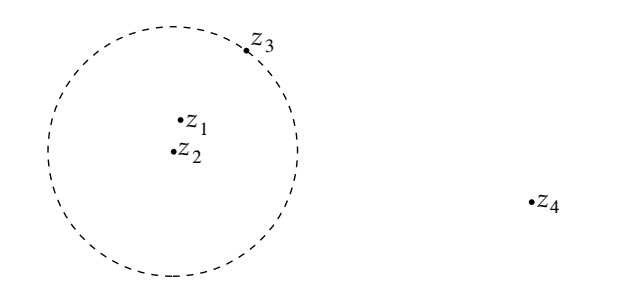
\includegraphics[width=0.6\textwidth,natwidth=400,natheight=180]{Fig2.1.jpg}
\caption{上图是四个定域算符的乘积. OPE将$z_1 \to z_2$时的渐近行为表示为一个级数. 其中$z_1 , z_2$处的一对算符被$z_2$处的单个算符代替. 收敛半径是它到其他最近算符的距离, 由图中的虚线表示.}\label{Fig2.1}
	\end{center}
\end{figure}

弦微扰论的基本研究对象是定域算符之积的路径积分期望值
\begin{equation}
\left\langle\mathscr{A}_{i_{1}}(z_{1}, \bar{z}_{1}) \mathscr{A}_{i_{2}}(z_{2}, \bar{z}_{2}) \cdots \mathscr{A}_{i_{n}}(z_{n}, \bar{z}_{n})\right\rangle
\end{equation}
其中$\mathscr{A}_{i}$是定域算符集合的某个基. 在其中两个算符互相接近彼此的极限下, 理解该期望值的行为是非常重要的. 给出该极限的系统描述是\emph{算符乘积展开}(OPE). 
如图\ref{Fig2.1}所示. 
OPE陈述为, 两个彼此接近的定域算符的乘积可以以任意精度被定域算符的和近似:
\begin{equation}
\mathscr{A}_{i}(\sigma_{1}) \mathscr{A}_{j}(\sigma_{2})=\sum_{k} c^{k}{}_{i j}(\sigma_{1}-\sigma_{2}) \mathscr{A}_{k}(\sigma_{2}) \:. \label{2.2.2}
\end{equation}
这是一个算符陈述, 意味着它在一个一般的期望值中成立
\begin{equation}
\left\langle\mathscr{A}_{i}(\sigma_{1}) \mathscr{A}_{j}(\sigma_{2}) \cdots\right\rangle
=\sum_{k} c^{k}{}_{i j}(\sigma_{1}-\sigma_{2})\left\langle\mathscr{A}_{k}\left(\sigma_{2}\right) \cdots\right\rangle \label{2.2.3}
\end{equation}
其中$\sigma_{1},\sigma_{2}$之间的间隔小于与其他所有算符的距离. 系数函数 $c^{k}{ }_{i j}(\sigma_{1}-\sigma_{2})$决定对间隔的依赖关系, 它也依赖于$i,j,k$, 但与期望值中的其他算符无关; 后者的依赖性仅出现在\eqref{2.2.3}右边的期望值中. 这些项通常的排列方法是:$\sigma_{1} \rightarrow \sigma_{2}$的极限下, 大小逐减. 除了系数函数不是简单的幂级数, 并可以在$\sigma_{1} \rightarrow \sigma_{2}$时奇异, 这类似于普通的Taylor级数.

我们现在将利用自由场论的特殊性质给出$X^\mu$理论的OPE推导. 在2.9节将给出任意共形不变场论的推导. 

我们已经看到, 正规乘积满足运动方程\eqref{2.1.23}. 这说明算符乘积是$(z_{1}, \bar{z}_{1})$的调和函数. 复变函数论中一个简单的结果是, 调和函数局域是一个全纯函数与一个反全纯函数之和. 特别地, 它意味着在$z_{1} \rightarrow z_{2}$时不奇异, 并且可以自由地用$z_{12}$和$\bar{z}_{12}$做Taylor展开. 因此,
\begin{align}
&X^{\mu}(z_{1}, \bar{z}_{1}) X^{v}(z_{2}, \bar{z}_{2})=-\frac{\alpha^{\prime}}{2} \eta^{\mu \nu} \ln \lvert z_{12}\rvert^{2}+ 
:\mathrel{ X^{v} X^{\mu}(z_{2}, \bar{z}_{2})}:  \nonumber \\
&\qquad +\sum_{k=1}^{\infty} \frac{1}{k!}\Bigl[(z_{12})^{k}\! :\mathrel{X^{v} \partial^{k} X^{\mu}(z_{2}, \bar{z}_{2})}:+
(\bar{z}_{12})^{k}\!:\mathrel{ X^{v} \bar{\partial}^{k} X^{\mu}(z_{2}, \bar{z}_{2})}:\Bigr] \label{2.2.4}
\end{align}
\begin{tcolorbox}
	\begin{remark}
		这里使用了\eqref{2.1.21a}和
	\begin{align*}
	&:\mathrel{X^{\mu}(z_{1},\bar{z}_{1}) X^{\nu}(z_{2}, \bar{z}_{2})}:\\
	=&: \mathrel{ X^{\nu} X^{\mu}(z_{2},\bar{z}_{2})}:+\sum_{k=1}^{\infty} \frac{1}{k !}\Bigl[(z_{12})^{k}\!:\mathrel{X^{\nu} \partial^{k} X^{\mu}(z_{2}, \bar{z}_{2})}:+(\bar{z}_{12})^{k}\!:\mathrel{X^{\nu} \bar{\partial}^{k} X^{\mu}(z_{2}, \bar{z}_{2})}:\Bigr]
	\end{align*}
	因为运动方程, 所以有混合导数$\partial \bar{\partial}$的项为零.
	\end{remark}
\end{tcolorbox}


方程\eqref{2.2.4}拥有OPE的形式. 就像导出它的运动方程\eqref{2.1.23}, 这是一个关于算符的陈述. 对于任何$X^{\mu}(z_{1},\bar{z}_{1}) X^{v}(z_{2},\bar{z}_{2})$于其它点处的场之积的真空期望值, 它在$z_{1}\to z_{2}$时的行为是一个无穷级数, 其中每一项都是$z_{12}$和(或) $\bar{z}_{12}$的已知函数乘以将这对场换成定域算符的期望值.

OPE通常被用作渐进展开, 前几项会在间隔很小时给出主导行为. 我们的大多数应用将是这类的, 我们通常将OPE写为明显奇异的项加上不明确指定的非奇异剩余项. 取代$=$, 我们将用“$\sim$”表示“在相差非奇异项的意义下相等”. 事实上, OPE在共形不变的场论中收敛. 在特定的应用中, 这对我们非常重要: 它使得从系数函数中重建整个理论变得可能. 作为一个例子, 自由场OPE \eqref{2.2.4}在任何给定期望值中的收敛半径等于路径积分中其它插入中距离它最近的那一个到它的距离, 如图\ref{Fig2.1}所示, 而收敛性可以通过标准复分析理论证明.

OPE \eqref{2.2.4}右边的各种算符包含同一个点处的场的乘积. 在量子场论中, 这样的乘积通常是发散的, 因而要被合适地截断并重整化, 但这里的正规编序使得它是的良好定义的. 
在自由场论中, 正规编序是一种定义复合算符的方便方法. 在相互作用场论中, 由于复合算符有来自于与其相连的相互作用顶点导致的额外发散, 所以正规编序的用处不大. 
然而我们感兴趣的场论大多是自由场论, 以及与自由场论相关的理论, 所以这里给出正规编序的更多细节.

任意多个场的正规编序可以递归地定义成
\begin{align}
&: \mathrel{ X^{\mu_{1}}(z_{1}, \bar{z}_{1}) \cdots X^{\mu_{n}}(z_{n}, \bar{z}_{n})}: \nonumber \\
&\qquad\quad =X^{\mu_{1}}(z_{1}, \bar{z}_{1}) \cdots X^{\mu_{n}}(z_{n}, \bar{z}_{n})+\sum \text{减除}, \label{2.2.5}
\end{align}
其中的减除项是指从场的乘积中挑出一对或多对场, 并将它们替换为$\frac{1}{2} \alpha^{\prime} \eta^{\mu_{i} \mu_{j}} \ln \lvert z_{i j}\rvert^{2}$. 例如,
\begin{align}
&:\mathrel{X^{\mu_{1}}(z_{1}, \bar{z}_{1}) X^{\mu_{2}}(z_{2}, \bar{z}_{2}) X^{\mu_{3}}(z_{3}, \bar{z}_{3})}: = 
X^{\mu_{1}}(z_{1}, \bar{z}_{1}) X^{\mu_{2}}(z_{2}, \bar{z}_{2}) X^{\mu_{3}}(z_{3}, \bar{z}_{3}) \nonumber \\
&\qquad+\left(\frac{\alpha^{\prime}}{2} \eta^{\mu_{1} \mu_{2}} \ln \lvert z_{12}\rvert^{2} X^{\mu_{3}}(z_{3}, \bar{z}_{3})+2 \text{ 个置换}\right). \label{2.2.6}
\end{align}

这个定义可以紧凑地总结为
\begin{equation}
: \mathrel{\mathscr{F}}:=\exp \left(\frac{\alpha^{\prime}}{4} \int \dif^{2} z_{1} \dif^{2} z_{2} \ln \lvert z_{12}\rvert^{2}\: 
\frac{\delta}{\delta X^{\mu}(z_{1}, \bar{z}_{1})} \frac{\delta}{\delta X_{\mu}(z_{2}, \bar{z}_{2})}\right) \mathscr{F} \:, \label{2.2.7}
\end{equation}
其中$\mathscr{F}$是$X$的任意泛函. 这等价于方程\eqref{2.2.5}: 指数中的双重求道会收缩每一对场, 而对任意多个配对的指数求和会与导数作用中的分数抵消. 这个形式表达式的一个应用是用指数的逆作用两边, 这样得到
\begin{align}
\mathscr{F} &=\exp \left(-\frac{\alpha^{\prime}}{4} \int \dif^{2} z_{1} \dif^{2} z_{2} \ln \lvert z_{12}\rvert^{2}\: 
\frac{\delta}{\delta X^{\mu}(z_{1}, \bar{z}_{1})} \frac{\delta}{\delta X_{\mu}(z_{2}, \bar{z}_{2})}\right):\mathrel{\mathscr{F}}: \nonumber \\
&=: \mathrel{\mathscr{F}}:+\sum \text {收缩}\:, \label{2.2.8}
\end{align}
其中收缩是减除的逆: 从$:\mathrel{\mathscr{F}}:$中挑出一对或多对场, 并将它们替换为$-\frac{1}{2} \alpha^{\prime} \eta^{\mu_{i} \mu_{j}} \ln \lvert z_{i j}\rvert^{2}$.

对$X$的任意泛函$\mathscr{F}$和$\mathscr{G}$, 它们的OPE由
\begin{equation}
: \mathrel{\mathscr{F}}: :\mathrel{\mathscr{G}}:=: \mathrel{\mathscr{F} \mathscr{G}}:+\sum \text{交叉收缩}
\end{equation}
生成. 现在是对$\mathscr{F}$中的一个场和$\mathscr{G}$的一个场配对收缩并求和. 这也可以写成
\begin{equation}
	: \mathrel{\mathscr{F}}: :\mathrel{\mathscr{G}}:= \exp \left(-\frac{\alpha^{\prime}}{2} 
	\int \dif^{2} z_{1} \dif^{2} z_{2}\: \ln \lvert z_{12}\rvert^{2} \frac{\delta}{\delta X_{F}^{\mu}(z_{1}, \bar{z}_{1})} 
	\frac{\delta}{\delta X_{G \mu}(z_{2}, \bar{z}_{2})}\right): \mathrel{\mathscr{F} \mathscr{G}}: \label{2.2.10}
\end{equation}
其中的泛函导数分别只作用在$\mathscr{F}$或$\mathscr{G}$中的场上.

作为一个例子,
\begin{align}
&: \mathrel{\partial X^{\mu}(z) \partial X_{\mu}(z)}: : \mathrel{\partial^{\prime} X^{v}(z^{\prime}) \partial^{\prime} X_{v}(z^{\prime})}: \nonumber \\
&\qquad \qquad \qquad =: \mathrel{\partial X^{\mu}(z) \partial X_{\mu}(z) \partial^{\prime} X^{v}(z^{\prime}) \partial^{\prime} X_{v}(z^{\prime})}: \nonumber\\
&\qquad \qquad \qquad \qquad \qquad {-}4 \cdot \frac{\alpha^{\prime}}{2}
(\partial \partial^{\prime} \ln \lvert z-z^{\prime}\rvert^{2}): \mathrel{\partial X^{\mu}(z) \partial^{\prime} X_{\mu}(z^{\prime})}: \nonumber\\
&\qquad \qquad \qquad \qquad \qquad {+}2 \cdot \eta^{\mu}{ }_{\mu}\left(-\frac{\alpha^{\prime}}{2} \partial \partial^{\prime}
 \ln \lvert z-z^{\prime}\rvert^{2}\right)^{2} \nonumber\\
 &\qquad \qquad \qquad \sim \frac{D \alpha^{\prime 2}}{2(z-z^{\prime})^{4}}-\frac{2 \alpha^{\prime}}{(z-z^{\prime})^{2}}
 : \mathrel{\partial^{\prime} X^{\mu}(z^{\prime}) \partial^{\prime} X_{\mu}(z^{\prime})}: \nonumber\\
&\qquad \qquad \qquad \qquad \qquad {-}\frac{2 \alpha^{\prime}}{z-z^{\prime}}: \mathrel{\partial^{\prime 2} X^{\mu}\left(z^{\prime}\right) \partial^{\prime} X_{\mu}\left(z^{\prime}\right)}:\:.  \label{2.2.11}
\end{align}
等号后的第二项来自与四种只收缩一对场的方法, 而第三项来自于两种收缩两对场的方法. 在最后一行我们通过在正规编序内部做Taylor展开把OPE写成标准形式: 每一项中的算符都在$z'$处, 并且按照奇异程度进行排列.

\begin{tcolorbox}
	\begin{remark}
		等号后的第二项来自于
	\begin{align*}
	\contraction{: \partial}{X^{\mu}}{(z) \partial X_{\mu}(z):: \partial^{\prime}}{X^{\nu}}: \mathrel{\partial  X^{\mu}(z) \partial X_{\mu}(z)}:
	: \mathrel{\partial^{\prime} X^{\nu} (z^{\prime}) \partial^{\prime} X_{\nu}(z^{\prime})}:  
	&=\partial \partial^{\prime}\left(-\frac{\alpha^{\prime}}{2} \eta^{\mu \nu}\ln \lvert z-z^{\prime}\rvert^{2}\right) 
	: \mathrel{\partial X_{\mu}(z) \partial X_{\nu}(z)}: \\
	&=-\frac{\alpha^{\prime}}{2} \Bigl(\partial \partial^{\prime} \ln \lvert z-z^{\prime}\rvert^{2}\Bigr)  
	: \mathrel{\partial X_{\mu}(z) \partial^{\prime} X^{\mu}(z)}:
	\end{align*}
	而第三项来自于
	\begin{align*}
	&\quad \contraction{: \partial}{X^{\mu}}{(z) \partial X_{\mu}(z):: \partial^{\prime}}{X^{\nu}}
	\bcontraction{: \partial X^\mu(z) \partial}{ X_\mu}{(z):: \partial^\prime X^\nu(z^\prime)\partial^\prime}{X_\nu}
		:\mathrel {\partial X^{\mu}(z) \partial X_{\mu}(z)}: : \mathrel{\partial^{\prime} X^{\nu}(z^{\prime}) \partial^{\prime} X_{\nu}(z^{\prime})}:\\
	&=\partial \partial^{\prime}\left(-\frac{\alpha^{\prime}}{2} \eta ^{\mu \nu} \ln \lvert z-z^{\prime}\rvert^{2}\right) 
	\partial \partial^{\prime}\left(-\frac{\alpha^{\prime}}{2} \eta_{\mu \nu}\ln \lvert z-z^{\prime}\rvert^{2}\right) \\
	&=\eta^{\mu \nu} \eta_{\mu \nu}\left(-\frac{\alpha^{\prime}}{2} \partial \partial^{\prime}\ln \lvert z- z^{\prime}\rvert ^{2}\right)^{2}
	\end{align*}
	因为$\eta^{\mu \nu} \eta_{\nu\rho}=\delta^{\mu}{}_{\rho}$, 所以$\eta^{\mu \nu} \eta_{\mu \nu}=\delta^{\mu}{ }_{\mu}=D$, 再利用
	$
	\partial \partial^{\prime} \ln \lvert z-z^{\prime }\vert ^{2}= (z-z^{\prime})^{-2}
	$
	和
	\[
	:\mathrel{\partial X^\mu(z)\partial^\prime X_{\mu}(z^\prime)}:\sim :\mathrel{\partial^\prime X^\mu(z^\prime)\partial^\prime X_\mu(z^\prime)}: 
	+ \:(z-z^\prime):\mathrel{\partial^{\prime 2} X^\mu(z^\prime)\partial^\prime X_\mu(z)}:
	\]
	就得到了\eqref{2.2.11}
	\end{remark}
\end{tcolorbox}


另一个重要的例子是
\begin{equation}
\mathscr{F}=\me^{\mi k_{1} \cdot X(z, \bar{z})}, \qquad \mathscr{G}=\me^{\mi k_{2} \cdot X(0,0)}
\end{equation}
变分$\delta / \delta X_{F}^{\mu}$和$\delta / \delta X_{G}^{\mu}$分别给出因子$\mi k_{1 \mu}$和$\mi k_{2 \mu}$, 所以一般结果\eqref{2.2.10}变成
\begin{align}
:\mathrel{\me^{\mi k_{1} \cdot X(z, \bar{z})}}: : \mathrel{\me^{\mi k_{2} \cdot X(0,0)}}: 
&=\exp \left(\frac{\alpha^{\prime}}{2} k_{1} \cdot k_{2} \ln |z|^{2}\right) :\mathrel{\me^{\mi k_{1} \cdot X(z, \bar{z})} \me^{\mi k_{2} \cdot X(0,0)}} : \nonumber \\
&=|z|^{\alpha^{\prime} k_{1} \cdot k_{2}}: \mathrel{ \me^{\mi k_{1} \cdot X(z, \bar{z})} \me^{\mi k_{2} \cdot X(0,0)}}: \:. \label{2.2.13}
\end{align}
为了推导OPE, 在正规编序中做Taylar展开给出
\begin{equation}
	:\mathrel{\me^{\mi k_{1} \cdot X(z, \bar{z})}}: : \mathrel{\me^{\mi k_{2} \cdot X(0,0)}}: 
	=|z|^{\alpha^{\prime} k_{1} \cdot k_{2}}: \mathrel{\me^{\mi(k_{1}+k_{2}) \cdot X(0,0)}[1+O(z, \bar{z})]}: \:.
\end{equation}
\begin{tcolorbox}[breakable]
	\begin{remark}
		一般结果\eqref{2.2.10}在这里是
	\begin{align*}
	&\quad :\mathrel{ \me^{i k_{1} \cdot X(z,\bar{z})}}::\mathrel{\me^{\mi k_{2} \cdot X(0,0)}}:\\
	&=\left(1-\frac{\alpha^{\prime}}{2} \int \dif^{2} z_{1} \dif^{2} z_{2}\: \ln \lvert z_{12}\rvert^{2} \frac{\delta}{\delta X_{F}^{\mu}(z_{1},\bar{z}_{1})} \frac{\delta}{\delta X_{G \mu}(z_{2}, \bar{z}_{2})} +\cdots \right):\mathrel{ \me^{\mi k_{1} \cdot X(z, \bar{z})} \me^{\mi k_{2} \cdot X(0,0)}}:\\
	&=:\mathrel{\me^{\mi k_{1} \cdot X(z, \bar{z})} \me^{\mi k_{2} \cdot X(0,0)}}: \\ 
	&\quad \times \left(1 -\frac{\alpha^{\prime}}{2} \int \dif^{2} z_{1} \dif^{2} z_{2}\: \ln \lvert z_{12}\rvert ^{2}
	 \times \mi k_{1 \mu} \delta^{2}(z-z_{1}, \bar{z}-\bar{z}_{1}) \mi k_{2}^{\mu} \delta^{2}(0-z_{2}, 0,-\bar{z}_{2})+ \cdots \right)\\
	&=:\mathrel{\me^{\mi k_{1} \cdot X(z, \bar{z})} \me^{\mi k_{2} \cdot X(0,0)}}: 
	\left(1+\frac{\alpha^{\prime}}{2} k_{1} \cdot k_{2} \ln |z|^{2}+\cdots\right)=
	|z|^{\alpha^{\prime} k_{1} \cdot k_{2}}: \mathrel{ \me^{\mi k_{1} \cdot X(z, \bar{z})} \me^{\mi k_{2} \cdot X(0,0)}}: \:.
	\end{align*}
	\end{remark}
\end{tcolorbox}

注意, OPE \eqref{2.2.2}, \eqref{2.2.4}等关于$\sigma_{1}$和$\sigma_{2}$是非对称的. 通过在$(\sigma_{1}+\sigma_{2})/ 2$附近做展开, 这些OPE可以重塑成对称的形式. 
对称形式下的系数函数在两个算符的交换下,
\begin{equation}
c^{k}{}_{ij}(\sigma_{1}-\sigma_{2})_{\mathrm{sym}}= \pm c^{k}{}_{j i}(\sigma_{2}-\sigma_{1})_{\mathrm{sym}} \:,
\end{equation}
其中, 当$\mathscr{A}_{i}$和$\mathscr{A}_{j}$都是反对易时符号取负号.


\section{\texorpdfstring{Ward恒等式与Noether定理}{2.3 Ward identities and Noether theorem}}

世界面对称性在弦论中扮演了一个重要角色. 在本节, 我们先导出对称性在场论中的一些普遍结果.

考察$d$维时空中作用量为$S_\phi$的一个场论, 其中用$\phi_\alpha(\sigma)$标记一般场. 设它有对称性
\begin{equation} \label{2.3.1}
\phi_{\alpha}^{\prime}(\sigma)=\phi_{\alpha}(\sigma)+\delta \phi_{\alpha}(\sigma) \:,
\end{equation}
其中$\delta \phi_\alpha$正比于无限小参量$\epsilon$. 路径积分测度与权重$exp(-S)$之积是不变的:
\begin{equation} \label{2.3.2}
	[\dif \phi^{\prime}]\: \exp(-S[\phi^{\prime}])=[\dif  \phi] \exp (-S[\phi]) \:.
\end{equation}

场论中, 连续对称性暗示着守恒流的存在(Noether定理), 以及Ward恒等式(其约束流的算符积). 为了导出这些结果, 考察场变分
\begin{equation}\label{2.3.3}
\phi_{\alpha}^{\prime}(\sigma)=\phi_{\alpha}(\sigma)+\rho(\sigma) \delta \phi_{\alpha}(\sigma)
\end{equation}
这不是对称性, $[\dif \phi]\mathrm{exp}(-S)$在$\rho$是一常量下不变, 所以它的变分必须正比于$\partial _a \rho$
\begin{align}
&[\dif \phi^{\prime}]\: \exp (-S[\phi^{\prime}]) \nonumber \\
&\qquad=[\dif \phi] \: \exp (-S[\phi])\left[1+\frac{\mi \epsilon}{2 \pi} \int \dif^{d} \sigma\: 
 g^{1 / 2} j^{a}(\sigma) \partial_{a} \rho(\sigma)+O\left(\epsilon^{2}\right)\right] \label{2.3.4}
\end{align}
未知系数$j^a(\sigma)$源于测度和作用量的变分. 仅在一个小区域里取$\rho$非零. 在区域之外, 考察含有一个一般插入``$\cdots$''的路径积分. 
这个插入在(\ref{2.3.3})下不变:
\begin{align}
0 &=\int[\dif \phi^{\prime}]\: \exp (-S[\phi^{\prime}]) \cdots \: - \: \int[\dif \phi] \exp (-S[\phi]) \cdots \nonumber \\
&=\frac{\epsilon}{2 \pi \mi} \int \dif^{d} \sigma \: g^{1 / 2} \rho(\sigma)\left\langle\nabla_{a} j^{a}(\sigma) \cdots\right\rangle
\label{2.3.5}
\end{align}
因而我们有
\begin{equation}
\nabla_{a} j^{a}=0 \:. \label{2.3.6}
\end{equation}
\begin{tcolorbox}
	\begin{remark}
		\eqref{2.3.6}的补充说明:
		\[
		\frac{\mi \epsilon}{2 \pi} \int \dif ^d \sigma\:g^{1 / 2} j^{a}(\sigma) \partial_{a} \rho(\sigma) 
		=\frac{\epsilon}{2 \pi \mi} \int \dif^{d} \sigma \: \partial_{a}(g^{1 / 2}j^{a})\rho(\sigma) \:,
		\]
		其中使用了 $\partial_{a}(g^{1 / 2} j^{a})=(\partial_{a} j^{a}) g^{1 / 2}+j^{a} (\partial_{a} g^{1 / 2})
		=g^{1 / 2}\nabla_{a}j^{a} \:$.
		\end{remark}	
\end{tcolorbox}

为了导出Ward等式, 令$\rho(\sigma)$在区域$R$内为1, 在$R$外为0. 另外在路径积分区域$R$内的一点$\sigma_{0}$处中引入一般定域算符$\mathscr{A}(\sigma_{0})$. 
在$R$外插入任意算符``$\cdots$''得到
\begin{equation} \label{2.3.7}
\delta \mathscr{A}(\sigma_{0})+\frac{\epsilon}{2 \pi \mi} \int_{R} \dif^{d} \sigma \: g^{1 / 2} \nabla_{a} j^{a}(\sigma) \mathscr{A}(\sigma_{0})=0 \:.
\end{equation}

\begin{tcolorbox}
	\begin{proof}
	类似于\eqref{2.3.5}, 我们现在有
	\[
	0=\int [\dif \phi]\:\me^{-S[\phi]}\biggl(\delta\mathscr{A}(\sigma_{0})+\frac{\mi\epsilon}{2\pi}\int \dif^{d}\sigma \: 
	j^{a}(\sigma)\partial_{a}\rho(\sigma)\mathscr{A}(\sigma_{0}) \biggr) \cdots	\:,
	\]
	然后利用分部积分就可以得到\eqref{2.3.7}.
	\end{proof}
	\end{tcolorbox}
\noindent 等价地, 
\begin{equation}
\nabla_{a} j^{a}(\sigma) \mathscr{A}(\sigma_{0})=g^{-1 / 2} \delta^{d}(\sigma-\sigma_{0}) \frac{2 \pi}{\mi \epsilon} \delta \mathscr{A}(\sigma_{0})+\sigma \:\text{的全导数} \:. \label{2.3.8}
\end{equation}
散度定理给出
\begin{equation}
\int_{\partial R} \dif A\: n_{a} j^{a} \mathscr{A}(\sigma_{0})=\frac{2 \pi}{\mi \epsilon} \delta \mathscr{A}(\sigma_{0}) \:,\label{2.3.9}
\end{equation}
其中$\dif A$是面积元, 而$n_{a}$是外法向量. 在2维平坦空间中, 这是
\begin{equation} \label{2.3.10}
\oint_{\partial R}(j\dif z-\tilde{\jmath} \dif \bar{z}) \mathscr{A}(z_{0}, \bar{z}_{0})
=\frac{2 \pi}{\epsilon} \delta \mathscr{A}(z_{0}, \bar{z}_{0})
\end{equation}
在这里我们扔掉了指标$j \equiv j_{z}$, $\tilde{\jmath} \equiv j_{\bar{z}}$. 我们使用$\tilde{\jmath}$而非$\bar{\jmath}$是因为$\tilde{\jmath}$并非$j$的共轭. 
Minkowski密度$j_0$一般是厄米的, $(j_{z})^{\dagger}=\frac{1}{2}(j_{1}-\mi j_{2})^{\dagger}=j_{z}$.
\begin{tcolorbox}
\begin{proof}
证明\eqref{2.3.9}使用了
\[
\int_{R} \dif^{d} \sigma \: g^{1 / 2} \nabla_{a} j^{a} =\int_{R} \dif ^{d} \sigma \: \partial_{a}\bigl(g^{1 / 2} j^{a}\bigr) 
=\int_{\partial R} \dif A\: n_{\alpha} j^{a} \:,
\]
利用二维的Stokes定理$
\int_{R} \dif^{2}z\: \bigl(\partial_{z} v^{z}+\partial_{\bar{z}} v^{\bar{z}}\bigr)=\mi \oint_{\partial R}(v^{z} \dif \bar{z}-v^{\bar{z}} \dif \bar{z})
$就得到了\eqref{2.3.10}.
\end{proof}
\end{tcolorbox}

重要的是Noether定理和Ward等式是定域性质, 并不依赖于远处的边界条件, 也不依赖在对称下是否不变. 特别的, 因为$\rho(\sigma)$仅在$R$内非零, 仅需要在$R$内定义对称变换.

在共形不变理论中, 通常$j_z$是全纯的, 而$j_{\bar{z}}$是反全纯的. 在这种情况下, 流$(j_z,0)$和$(0,j_{\bar{z}})$分别守恒. 于是积分给出OPE中的留数:
\begin{equation}\label{2.3.11}
\operatorname{Res}_{z \to z_{0}} j(z) \mathscr{A}(z_{0}, \bar{z}_{0})+\overline{\operatorname{Res}}_{\bar{z} \to \bar{z}_{0}} \, \tilde{\jmath}(\bar{z}) \mathscr{A}(z_{0}, \bar{z}_{0})=\frac{1}{\mi \epsilon} \delta \mathscr{A}(z_{0}, \bar{z}_{0})
\end{equation}
这里$\operatorname{Res},\overline{\operatorname{Res}}$分别是指取$(z-z_{0})^{-1}$和$(\bar{z}-\bar{z}_{0})^{-1}$的系数.

一个例子:回到无质量自由标量场, 并考虑考虑\emph{时空}平移$\delta X^{\mu}=\epsilon a^{\mu}$. 在$\delta X^{\mu}(\sigma)=\epsilon \rho(\sigma) a^{\mu}$ 下,
\begin{align}
\delta S=\frac{1}{4 \pi \alpha^{\prime}} \int \dif^{2}\sigma\: 2(\delta \partial^{a} X^{\mu}) \partial_{a} X_{\mu} 
=\frac{\epsilon a_{\mu}}{2 \pi \alpha^{\prime}} \int \dif^{2} \sigma \:\partial^{a} X^{\mu} \partial_{a} \rho \:.
\end{align}
这相当于把\eqref{2.3.5}中的Noether流取成$j_{a}(\sigma)=a_{\mu} j_{a}^{\mu}$, 其中
\begin{equation}
j_{a}^{\mu}=\frac{\mi}{\alpha^{\prime}} \partial_{a} X^{\mu} \:. \label{2.3.13}
\end{equation}
流与指数算符的OPE给出
\begin{subequations} \label{2.3.14}
\begin{align}
j^{\mu}(z): \mathrel{\me^{\mi k \cdot X(0,0)}}: &\sim \frac{k^{\mu}}{2 z}: \mathrel{\me^{\mi k \cdot X(0,0)}}:  \:,\label{2.3.14a} \\
\tilde{\jmath}^{\mu}(\bar{z}):\mathrel{ \me^{\mi k \cdot X(0,0)}}: &\sim \frac{k^{\mu}}{2 \bar{z}}: 
\mathrel{\me^{\mi k \cdot X(0,0)}}:\:. \label{2.3.14b}
\end{align}
\end{subequations}
\begin{tcolorbox}
	\begin{proof}
		\eqref{2.3.14a}的说明:由\eqref{2.3.13}可以得出$j^{\mu}=j_{z}^{\mu}=\frac{\mi}{\alpha^{\prime}} \partial_{z} X^{\mu}$, 所以
		\begin{align*}
			\frac{\mi}{\alpha^{\prime}} \partial_{z} X^{\mu} : \mathrel{\me^{\mi k \cdot X(0,0)}}: \sim 
			\mi k_{\nu}\frac{\mi}{\alpha^{\prime}} \partial_{z} \langle X^{\mu}(z,\bar{z})X^{\nu}(0,0)\rangle : \mathrel{\me^{\mi k \cdot X(0,0)}}: 
			=\frac{k^{\mu}}{2 z}: \mathrel{\me^{\mi k \cdot X(0,0)}}:
		\end{align*}
		\end{proof}
\end{tcolorbox}

另一例子: 世界面平移$\delta \sigma^{a}=\epsilon v^{a}$, 这时$\delta X^{\mu}=-\epsilon v^{a} \partial_{a} X^{\mu}$, Noether流是
\begin{subequations}
\begin{align}
j_{a}  &=\mi v^{b} T_{a b} \:, \label{2.3.15a} \\
T_{a b}&=-\frac{1}{\alpha^{\prime}}:\mathrel{\biggl(\partial_{a} X^{\mu} \partial_{b} X_{\mu}-\frac{1}{2} \delta_{a b} \partial_{c} X^{\mu} \partial^{c} X_{\mu}\biggr)}: \:. \label{2.3.15b}
\end{align}
\end{subequations}

% \begin{proof}
% (2.3.15a)的证明:
% $$
% \delta \sigma^{u}=\epsilon v^{a}, \quad \delta X^{\mu}=-\partial_{a} X^{\mu} \delta \sigma^{a}=-\epsilon v^{a} \partial_{a} X^{\mu}
% $$
% $$
% \begin{aligned}
% \delta S &=\frac{1}{4 \pi \alpha^{\prime}} \int d^{2} \sigma 2 \delta \partial^{\alpha} X^{\mu} \partial_{a} X_{\mu} \\
% &=-\frac{1}{2 \pi \alpha^{\prime}} \int d^{2} \sigma \delta X^{\mu} \partial^{a} \partial_{a} X_{\mu} \\
% &=-\frac{1}{2 \pi \alpha^{\prime}} \int d^{2} \sigma\left(-\epsilon v^{a} \partial_{\alpha} X^{\mu}\right) \rho(\sigma) \partial^{\alpha} \partial_{a} X_{\mu} \\
% &=\frac{\epsilon v^{\alpha}}{2 \pi \alpha^{\prime}} \int d^{2} \sigma  \partial_{a} X^{\mu} \rho(\sigma) \partial^{b} \partial_{b} X_{u}
% \end{aligned}
% $$
% $$
% \begin{array}{l}
% \int d^{2} \sigma \partial_{b}\left(\partial_{a} X^{\mu} \rho(\sigma)\right) \partial^{b} X_{u} \\
% =\int d^{2} \sigma  \partial_{a} X^{\mu} \partial^{b} X_{\mu} \partial_{b} \rho(\sigma)+\rho(\sigma) \partial_{b} \partial_{a} X^{\mu} \partial^{b} X_{\mu}\\
% =\int d^{2} \sigma \partial_{a} X^{\mu} \partial^{b} X_{\mu} \partial_{b} \rho(\sigma)-\partial_{a} \rho(\sigma) \partial_{b} X^{\mu} \partial^{b} X_{\mu}-\rho(\sigma) \partial_{a} X^{\mu} \partial_{b} \partial^{b} X^{\mu} \\
% =\int d^{2} \sigma \partial_{a} X^{\mu} \rho(\sigma) \partial^{b} \partial_{b} X^{\mu} \\
% =\frac{1}{2} \int d^{2} \sigma \partial_{a} X^{\mu} \partial^{b} X_{\mu} \partial_{b} \rho(\sigma)-\partial_{a} \rho(\sigma) \partial_{b} X^{\mu} \partial^{b} X_{u}
% \end{array}
% $$
% $$
% \frac{\epsilon v^{a}}{2 \pi \alpha^{\prime}} \int d^{2} \sigma \frac{1}{2} \left[\partial_{a} X^{\mu} \partial^{b} X_{\mu} \partial_{b} \rho(\sigma)-\partial_{a}\rho \partial_{b} X^{\mu}  \partial^{b} X_{\mu}\right]=\frac{i \epsilon}{2 \pi} \int d^{2} z j^{a}(\sigma) \partial_{a}(\rho)
% $$
% \end{proof}


\section{\texorpdfstring{共形不变性}{2.4 Conformal invariance}}

能动量张量\eqref{2.3.15b}无迹: $T_a{}^a=0$. 在复坐标中, 这是
\begin{equation}
T_{z \bar{z}}=0\:. \label{2.4.1}
\end{equation}
守恒律$\partial^a T_{ab}=0$暗示着在任何$T_a{}^a=0$的理论中
\begin{equation}
\bar{\partial} T_{z z}=\partial T_{\bar{z} \bar{z}}=0 \:. \label{2.4.2}
\end{equation}
因此
\begin{equation}
T(z) \equiv T_{z z}(z)\:, \qquad \tilde{T}(\bar{z}) \equiv T_{\bar{z} \bar{z}}(\bar{z}) \label{2.4.3}
\end{equation}
分别是全纯的和反全纯的. 对于无质量自由标量
\begin{equation}\label{2.4.4}
T(z)=-\frac{1}{\alpha^{\prime}}: \mathrel{\partial X^{\mu} \partial X_{\mu}}: \:, \qquad 
\tilde{T}(\bar{z})=-\frac{1}{\alpha^{\prime}}:\mathrel{ \bar{\partial} X^{\mu} \bar{\partial} X_{\mu}}: \:,
\end{equation}
根据运动方程, 它们确实是全纯和反全纯的.


$T_{ab}$的无迹暗示着一个大得多的对称性. 流
\begin{equation}
j(z)=\mi v(z) T(z) \:, \qquad \tilde{\jmath}(\bar{z})=\mi v(z)^{*} \tilde{T}(\bar{z}) \label{2.4.5}
\end{equation}
对于全纯的$v(z)$是守恒的.
\begin{tcolorbox}
	\begin{proof}
		记$j_{z}=i v^{z} T_{z z}$, $j_{\bar{z}}=i v^{\bar{z}} T_{\bar{z} \bar{z}}$. 所以$
		\nabla_{a} j^{a}= \bar{\partial} j_{z}+\partial j_{\bar{z}}=0$.
		\end{proof}	
\end{tcolorbox}
对于自由标量理论, 得到OPE
\begin{equation} \label{2.4.6}
T(z) X^{\mu}(0) \sim \frac{1}{z} \partial X^{\mu}(0), \quad \tilde{T}(\bar{z}) X^{\mu}(0) \sim \frac{1}{\bar{z}} \bar{\partial} X^{\mu}(0)
\end{equation}
% \begin{proof}
% $$
% T(z)=-\frac{1}{\alpha^{\prime}}: \partial X^{\mu} \partial X_{\mu}:
% $$
% $$
% -\frac{1}{\alpha^{\prime}}: \partial X^{\mu} \partial X_{\mu}: X^{\nu}(0)=-\frac{1}{\alpha^{\prime}}: \partial X^{\mu} \partial X_{\mu}(z) X^{\nu}(0):\sim \frac{1}{z} \partial X_{\mu} (0)
% $$
% \end{proof}
那么Ward恒等式给出变换
\begin{equation}\label{2.4.7}
\delta X^{\mu}=-\epsilon v(z) \partial X^{\mu}-\epsilon v(z)^{*} \bar{\partial} X^{\mu}
\end{equation}
这是无限小坐标变换$z^{\prime}=z+\epsilon v(z)$. 
有限变换是
\begin{equation} \label{2.4.8}
X^{\prime \mu}\left(z^{\prime}, \bar{z}^{\prime}\right)=X^{\mu}(z, \bar{z}), \quad \text{其中 }z^{\prime}=f(z) \:.
\end{equation}
\eqref{2.4.8}被称为\emph{共形变换}.
\begin{tcolorbox}
		关于\eqref{2.4.7}的证明: 由(\ref{2.3.11})
		$$
		\frac{1}{\mi \epsilon} \delta X^{\mu}=\operatorname{Res}_{z \rightarrow z_{0}} \mi v^{z} T(z) X^{\mu}(z_{0},\bar{z}_{0})+
		\overline{\operatorname{Res}}_{\bar{z} \rightarrow \bar{z}_{0}} \mi v^{\bar{z}} \bar{T}(\bar{z}) X^{\mu}(z_{0},\bar{z}_{0})
		$$
		利用\eqref{2.4.6}就得到了\eqref{2.4.7}.
\end{tcolorbox}


共形不变性不应与diff不变性相混淆. 我们处在平坦空间中, 没有独立的度规场用来做变分. 所以变换$z\to z^\prime$真的改变了点的距离. 我们不是随随便便就有了这种不变性; 它是关于动力学的非平庸陈述. 对于标量作用量\eqref{2.1.10}, $\partial$和$\bar{\partial}$的共形变换恰好与$\dif^2 z$的共形变换抵消. 质量项$m^{2} X^{\mu} X_{\mu}$则不是共形不变的.
最终, 这里必然有一个与 Polyakov 弦的 diff$\times$ Weyl 对称性的紧密联系.

考虑特殊情况
\begin{equation}\label{2.4.9}
z^{\prime}=\zeta z \:,
\end{equation}
$\zeta$为任意复数. $\zeta$的相位是系统的旋转, 它的大小则是系统尺寸的重新标度. 这种标度不变性通常视为粒子物理中的一个近似对称性, 在临界点附近的统计系统也是由标度不变的场论描述.

对于广义共形变换, 考察它在$\dif s^{2}=g_{ab}\dif\sigma^{a} \dif \sigma^{b}=\dif z \dif \bar{z}$ 上的效应
\begin{equation}
\dif s^{\prime 2}=\dif z^{\prime} \dif \bar{z}^{\prime}=\frac{\partial z^{\prime}}{\partial z} \frac{\partial \bar{z}^{\prime}}{\partial \bar{z}} \dif z \dif \bar{z} \:.
\end{equation}
如图\ref{fig2.2}所示, 我们看到共形变换将无限小平方变为无限小平方但调节了大小. 一个反全纯函数$z^{\prime}=f(z)^{*}$有相同的性质但改变了定向. 
在(\ref{2.4.9})下不变的大多数系统通常在大得多的共形不变性下不变. 有这种不变性的理论称为\emph{共形场论}(CFT). 
\begin{figure}[h]
	\begin{center}
		%	\includegraphics[width=0.8\textwidth,bb=0 0 803 312]{Fig2.3ClosedStringCoordinates.jpg}\\
		%1px=0.75pt
		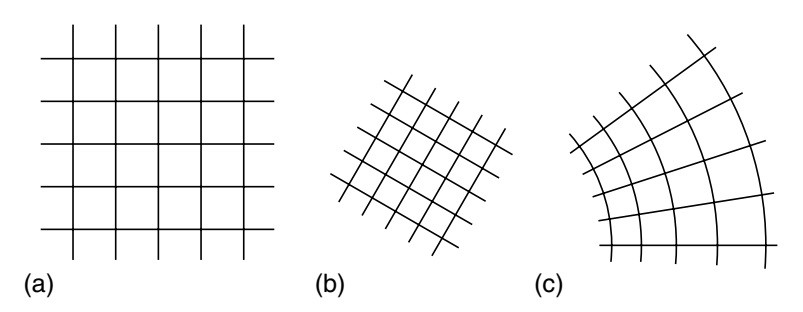
\includegraphics[width=0.8\textwidth,natwidth=520,natheight=200]{Fig2.2.jpg}
\caption{(a) 二维区域. (b) 特殊共形变换\eqref{2.4.9}的效应. (c) 更一般共形变换的效应.} \label{fig2.2}
	\end{center}
\end{figure}

\subsection*{共形不变与OPE}

共形不变给 OPE 的形式施加了一个很强的约束, 尤其是能动量张量的 OPE. 考察$T$与一般算符$\mathscr{A}$的OPE. 因为$T(z)$和 $\tilde{T}(\bar{z})$除了相交点以外是(反)全纯的, 相应的系数函数也要有这个性质. $T$与$\mathscr{A}$的OPE因而是Laurent展开, 展开项是z的整数次幂, 但次数可能为负. 更进一步, 所有奇异项都由$\mathscr{A}$的共形变换决定. 为了看到这一点, 我们写出奇异性的一般展开
\begin{equation}\label{2.4.11}
T(z) \mathscr{A}(0,0) \sim \sum_{n=0}^{\infty} \frac{1}{z^{n+1}} \mathscr{A}^{(n)}(0,0)
\end{equation}
与$\tilde{T}$相似; 算符系数$\mathscr{A}^{(n)}$留到以后决定. 在无限小共形变换$z^{\prime}=z+\epsilon v(z)$下, 当$T \mathscr{A}$ OPE中的$z^{-n-1}$ 项与$v(z)$中 $z^n$项相乘时, $v(z) T(z) \mathscr{A}(0,0)$ 中会出现一个单极点. 因此 Ward 恒等式的(\ref{2.3.11})形式暗示
\begin{equation}\label{2.4.12}
\delta \mathscr{A}(z, \bar{z})=-\epsilon \sum_{n=0}^{\infty} \frac{1}{n !}\Bigl[\partial^{n} v(z) \mathscr{A}^{(n)}(z, \bar{z})+\bar{\partial}^{n} v(z)^{*} \tilde{\mathscr{A}}^{(n)}(z, \bar{z})\Bigr]
\end{equation}
因此算符$\mathscr{A}^{(n)}$ 由$\mathscr{A}$的共形变换决定. 

取在刚性变换(\ref{2.4.9})下为本征态的算符为基是方便的
\begin{equation}\label{2.4.13}
\mathscr{A}^{\prime}(z^{\prime}, \bar{z}^{\prime})=\zeta^{-h} \bar{\zeta}^{-\tilde{h}} \mathscr{A}(z, \bar{z}) \:.
\end{equation}
$(h, \tilde{h})$称为权重. $h+ \tilde{h}$是$\mathscr{A}$的维数, 决定了$\mathscr{A}$在重新标度下的行为, 而$h- \tilde{h}$是自旋, 决定它在旋转下的行为. 导数$\partial_z$ 提升 $h$ 一次,   $\partial_{\bar{z}}$ 提升 $\tilde{h}$ 一次. 变换(\ref{2.4.13})的Ward恒等式与平移$\delta \mathscr{A}=-\epsilon v^{a} \partial_{a} \mathscr{A}$ 的Ward等式决定了OPE的部分
\begin{equation}\label{2.4.14}
T(z) \mathscr{A}(0,0)=\cdots+\frac{h}{z^{2}} \mathscr{A}(0,0)+\frac{1}{z} \partial \mathscr{A}(0,0)+\cdots
\end{equation}
对$\tilde{T}$类似.
\begin{tcolorbox}
	\begin{remark}
		变换\eqref{2.4.13}造成的变分是
		\begin{align*}
		\delta \mathscr{A} =\mathscr{A}^{\prime}(z, \bar{z})-\mathscr{A}(z, \bar{z}) 
		=\mathscr{A}^{\prime}(z^{\prime} / \zeta, \bar{z}^{\prime} / \zeta)-\mathscr{A} ( z, \bar{z})
		\end{align*}
		令$\zeta=1+\epsilon v$, 那么$z^{\prime} / (1+\epsilon v)=z^{\prime}(1-\epsilon v)$
		则
		$$
		\begin{aligned}
		\delta \mathscr{A} &=\mathscr{A}^{\prime}(z^{\prime}, \bar{z}^{\prime})-\epsilon v z^{\prime} \partial \mathscr{A}^{\prime}\left(z^{\prime}\right)-\epsilon \bar{v}{\bar{z}^{\prime}} \bar{\partial} \mathscr{A}^{\prime}(\bar{z}^{\prime})-\mathscr{A}(z, \bar{z}) \\
		&=[(1+\epsilon v)^{h}(1+\epsilon\bar{v})^{-h} -1] \mathscr{A}  
		-\epsilon v z^{\prime} \partial \mathscr{A}^{\prime}(z^{\prime})-\epsilon \bar{v} \bar{z}^{\prime} \bar{\partial} \mathscr{A}^{\prime}(\bar{z}^{\prime})
		\end{aligned}
		$$
		\end{remark}
\end{tcolorbox}

一个特别重要的是张量算符或基础场$\mathcal{O}$.  一般的共形变换作用其上给出
\begin{equation}
\mathcal{O}^{\prime}(z^{\prime}, \bar{z}^{\prime})= (\partial_{z} z^{\prime})^{-h}(\partial_{\bar{z}} \bar{z}^{\prime})^{-\tilde{h}} \mathcal{O}(z, \bar{z}) \:.
\end{equation}
OPE \eqref{2.4.11}约化成
\begin{equation}\label{2.4.16}
T(z) \mathcal{O}(0,0)=\frac{h}{z^{2}} \mathcal{O}(0,0)+\frac{1}{z} \partial \mathcal{O}(0,0)+\cdots \:,
\end{equation}
一般OPE(\ref{2.4.14})中更加奇异的项没有了.

再一次取自由$X^\mu$ CFT 为例子. 一些典型算符的权重是
\begin{equation}
\left.\begin{array}{llll}
X^{\mu} & (0,0) \:, & \partial X^{\mu} & (1,0) \:, \\
\bar{\partial} X^{\mu} & (0,1) \:, & \partial^{2} X^{\mu} & (2,0)  \:,\\
: \mathrel{\me^{\mi k \cdot X}}: & \left(\frac{\alpha^{\prime} k^{2}}{4}, \frac{\alpha^{\prime} k^{2}}{4}\right) \:. & &
\end{array}\right\} \label{2.4.17}
\end{equation}
除了$\partial^{2} X^{\mu}$, 所有量都按张量变换. 更一般地, 指数与导数的一般乘积
\begin{equation}
:\mathrel{\Bigl({\textstyle \prod_{i}} \partial^{m_{i}} X^{\mu_{i}}\Bigr)\Bigl({\textstyle \prod_{j}} \bar{\partial}^{n_{j}} X^{v_{j}}\Bigr) \me^{\mi k \cdot X} }:
\end{equation}
具有权重
\begin{equation}
\biggl(\frac{\alpha^{\prime} k^{2}}{4}+ {\textstyle\sum_{i}} m_{i}, \frac{\alpha^{\prime} k^{2}}{4}+\textstyle{\sum_{j}} n_{j}\biggr) \:. \label{2.4.19}
\end{equation}

对于任意一对算符, 在OPE两边作用刚性变换, 重新标度与旋转完全决定系数函数对$z$的依赖
\begin{equation}\label{2.4.20}
\mathscr{A}_{i}(z_{1}, \bar{z}_{1}) \mathscr{A}_{j}(z_{2}, \bar{z}_{2})=\sum_{k} z_{12}^{h_{k}-h_{i}-h_{j}} 
\bar{z}_{12}^{\tilde{h}_{k}-\tilde{h}_{i}-\tilde{h}_{j}} c^{k}{}_{i j} \mathscr{A}_{k}(z_{2}, \bar{z}_{2}) \:,
\end{equation}
其中$c^k{}_{ij}$ 现在是一常数. 在所有感兴趣的情况中, OPE(\ref{2.4.20})右边出现的权重有下界, 所以算符乘积中的奇异度被约束住了. 更普遍的共形变换在 OPE 上施加了进一步的约束:它们用基础场的 OPE 完全决定了所有场的 OPE.

注意, 一般而言, 正规乘积(normal ordered
products)的共形变换性质不由乘积的朴素(naive)变换决定. 例如, $X^\mu$的变换法则(\ref{2.4.7})将朴素地暗示
\begin{equation}
\delta \me^{\mi k \cdot X}=-\epsilon v(z) \partial \me^{\mi k \cdot X}-\epsilon v(z)^{*} \bar{\partial} \me^{\mi k \cdot X} \quad \text { (naive) }
\end{equation}
使其成为(0,0)张量. 由于在一点定义算符乘积需要重整化, 这个修正是量子效应. 特别地, 它进入这里是因为在$\mathrel{:\::}$中减除$\ln \lvert z_{12}\rvert^{2}$ 会对坐标系有明显的依赖. 

\subsection*{能动量张量的共形性质}
能动量张量与其自身的OPE由\eqref{2.2.11}获得
\begin{equation}\label{2.4.22}
\begin{aligned}
T(z) T(0) &=\frac{\eta^{\mu}{}_{\mu}}{2 z^{4}}-\frac{2}{\alpha^{\prime} z^{2}}: \mathrel{\partial X^{\mu}(z) \partial X_{\mu}(0)}:+ 
: \mathrel{T(z) T(0)}: \\
& \sim \frac{D}{2 z^{4}}+\frac{2}{z^{2}} T(0)+\frac{1}{z} \partial T(0)
\end{aligned}
\end{equation}
对于$\tilde{T}$有一个类似结果. 
$T(z) \tilde{T}(\bar{z}^{\prime})$的OPE必须是非奇异的, 它不可能在$(z-z^{\prime})$处有奇点, 这是因为它在非零间隔上对$z^{\prime}$ 是反全纯的. 类似地, 它不可能在$(\bar{z}-\bar{z}^{\prime})$处有奇点. 相同结果对于一个全纯算符和一个反全纯算符的任何OPE成立. 

因此$T$\emph{不}是一个张量. 而OPE \eqref{2.4.22}暗示了变换规则
\begin{equation}
\epsilon^{-1} \delta T(z)=-\frac{D}{12} \partial_{z}^{3} v(z)-2 \partial_{z} v(z) T(z)-v(z) \partial_{z} T(z) \:. \label{2.4.23}
\end{equation}
在一个一般的CFT中,  $T(z)$的变换
\begin{equation}\label{2.4.24}
\epsilon^{-1} \delta T(z)=-\frac{c}{12} \partial_{z}^{3} v(z)-2 \partial_{z} v(z) T(z)-v(z) \partial_{z} T(z) \:,
\end{equation}
其中$c$是被称为中心荷的常数. 自由标量场的中心荷是1. 对于$D$个自由标量场则是$D$. 变换(\ref{2.4.24})是最普遍的形式, 其对$v$是线性的. 这与$TT$ OPE的对称性是一致的, 其中3个$z$下标是刚性变换、重新标度和旋转不变性要求的. 标度、旋转和平移对称性决定了第2项和第3项的系数. 进一步地, 通过考察两个这样变换的对易子, 可以证明$\partial_{a} c=0$. 这是量子场论中的一个普遍结果. 独立于位置的算符必须是c数. 相对应的$TT$ OPE是
\begin{equation}\label{2.4.25}
T(z) T(0) \sim \frac{c}{2 z^{4}}+\frac{2}{z^{2}} T(0)+\frac{1}{z} \partial T(0)
\end{equation}
变换规则(\ref{2.4.24})的有限形式是
\begin{equation}\label{2.4.26}
(\partial_{z} z^{\prime})^{2} T^{\prime}(z^{\prime})=T(z)-\frac{c}{12}\{z^{\prime}, z\} \:,
\end{equation}
其中$\{f,z\}$代表Schwarzian 导数
\begin{equation}
\{f, z\}=\frac{2 \partial_{z}^{3} f \partial_{z} f-3 \partial_{z}^{2} f \partial_{z}^{2} f}{2 \partial_{z} f \partial_{z} f}
\end{equation}
对于$\tilde{T}$有相应形式. 在一般CFT中可能会有一个不同的中心荷$\tilde{c}$.
能动量张量的非张量行为有几个重要的物理结果. 应该强调的是, ``非张量''指代的是共形变换. 在坐标变换下, 能动量张量将具有通常的张量性质.

\section{\texorpdfstring{自由共形场论}{2.5 Free CFTs}} \label{sec:2.5}
在本节, 我们将讨论三类自由场CFT——线性伸缩子理论, $bc$理论与$\beta\gamma$理论. $bc$理论将在下一章用来规范固定Polyakov弦. 这三个理论都有广泛的应用.

\subsection*{线性伸缩子CFT}

这类CFT基于同一作用量\eqref{2.1.10}. 但能动张量是
\begin{subequations} \label{2.5.1}
\begin{align}
T(z)&=-\frac{1}{\alpha^{\prime}}: \mathrel{\partial X^{\mu} \partial X_{\mu}}:+ V_{\mu} \partial^{2} X^{\mu} \label{2.5.1a} \\
\tilde{T}(\bar{z})&=-\frac{1}{\alpha^{\prime}}: \mathrel{\bar{\partial} X^{\mu} \bar{\partial} X_{\mu}}:+V_{\mu} \bar{\partial}^{2} X^{\mu}
\label{2.5.1b}
\end{align}
\end{subequations}
其中$v_\mu$是某个固定的$D$-矢量. 算出$TT$ OPE, 就会发现它正是标准形式(\ref{2.4.25}). 但中心荷为
\begin{equation}
c=\tilde{c}=D+6 \alpha^{\prime} V_{\mu} V^{\mu}
\end{equation}
$TX^\mu $ OPE与 Ward 恒等式(\ref{2.4.12})暗示着共形变换
\begin{equation}
\delta X^{\mu}=-\epsilon v \partial X^{\mu}-\epsilon v^{*} \bar{\partial} X^{\mu}-\frac{\epsilon}{2} \alpha^{\prime} V^{\mu}\left[\partial v+(\partial v)^{*}\right]
\end{equation}
这是同一作用量不同的共形对称性. $X^\mu$不再按照一个张量变换, 它的变分现在有非齐次部分. 附带的, 二维中的自由无质量标量有一大类对称性——比我们偶然提及的要多得多. 

能动量张量在弦论中扮演了一个特殊的角色. 尤其是, 它告诉我们如何与一弯曲度规耦合——$V^\mu$的不同值可以视为不同的CFT. 矢量$V^\mu$选出了时空中的一个方向, 因而这个CFT不是Lorentz不变的, 我们对此没什么兴趣. 在3.7节我们将看到线性伸缩子CFT的一个物理解释, 并在稍后的某些技巧性应用中遇到它. 自由标量CFT的一个不同变分是取某些  $X^\mu$为周期的;我们将在第8章着手处理它.
%\centerline{\Large bc CFT}

\subsection*{$bc$ CFT}
第二类CFT有反对易场b和c, 以及作用量
\begin{equation}\label{2.5.4}
S=\frac{1}{2 \pi} \int \dif^{2} z\:  b \bar{\partial} c \:. 
\end{equation}
对于任意给定的常数$\lambda$, 使得
\begin{equation}
h_{b}=\lambda, \quad h_{c}=1-\lambda
\end{equation}
若$b$和$c$像权重$\left(h_{b}, 0\right)$ 和 $\left(h_{c}, 0\right)$ 的张量那样变换, (\ref{2.5.4})是共形不变的, 因而我们有另一类CFT(我们将在第10章看到, 其暗底里与线性伸缩子是相同的). 可以通过相同的方法\eqref{2.1.15}、\eqref{2.1.18}获得运动的算符方程
\begin{subequations} \label{2.5.6}
\begin{align}
\bar{\partial} c(z) &=\bar{\partial} b(z)=0  \label{2.5.6a} \\
\bar{\partial} b(z) c(0) &=2 \pi \delta^{2}(z, \bar{z})  \label{2.5.6b} 
\end{align}
\end{subequations}
$bb$ OPE与$cc$ OPE满足无源运动方程. $bc$的正规乘积是
\begin{equation}\label{2.5.7}
: \mathrel{b(z_{1}) c(z_{2})}:=b(z_{1}) c(z_{2})-\frac{1}{z_{12}}
\end{equation}
由于
\begin{equation}
\bar{\partial} \frac{1}{z}=\partial \frac{1}{\bar{z}}=2 \pi \delta^{2}(z, \bar{z})
\end{equation}
(\ref{2.5.7})满足朴素的运动方程. (\ref{2.5.7})可以通过对一包含原点的区域积分, 并分部积分得到. 场的普通乘积的正规序在组合学上与$X^\mu$ CFT相同, 是收缩或减除之和. 
我们必须小心: 由于$b$和$c$是反对易的, 所以场的交换会翻转符号.  

算符乘积是
\begin{equation}
b(z_{1}) c(z_{2}) \sim \frac{1}{z_{12}}, \qquad c(z_{1}) b(z_{2}) \sim \frac{1}{z_{12}}
\end{equation}
在第二个OPE中进行过两次符号反转, 一个来源于反对易, 一个来自$z_{1} \leftrightarrow z_{2}$. 其他算符乘积是非奇异的:
\begin{equation}
b(z_{1}) b(z_{2})=O(z_{12}) \:, \qquad c(z_{1}) c(z_{2})=O(z_{12}) \:.
\end{equation}
这些不仅是全纯的, 并且由于反对称性有一零点.

Noether定理给出能动量张量
\begin{subequations}\label{2.5.11}
\begin{align}
T(z)&=:\mathrel{(\partial b) c}:-\lambda \partial(: \mathrel{b c}:)  \:,  \label{2.5.11a}\\
\tilde{T}(\bar{z})&=0  \:. \label{2.5.11b}
\end{align}
\end{subequations}
通过给出$T$与$b$和$T$与$c$的OPE, 可以证明(\ref{2.5.11}), 它有权重给定的标准张量形式(\ref{2.4.16}). $TT$ OPE是标准形式(\ref{2.4.25}). 其中
\begin{equation}
c=-3(2 \lambda-1)^{2}+1\:, \qquad \tilde{c}=0 \:. \label{2.5.12}
\end{equation}
这是一个纯粹的全纯CFT, 也是一个$c \neq \tilde{c}$的例子. 当然有一相应的反全纯理论
\begin{equation}
S=\frac{1}{2 \pi} \int \dif^{2} z \: \tilde{b} \partial \tilde{c} \:,
\end{equation}
在$z \leftrightarrow \bar{z}$ 下, 这与之上是相同的.

$bc$理论有一鬼数对称性$\delta b=-\mi \epsilon b, \delta c=\mi \epsilon c$. 对应的Noether流
\begin{equation}\label{2.5.14}
j=-:\mathrel{b c}:
\end{equation}
分量分别是全纯的和反全纯的, 后者为0. 当既有全纯bc场, 又有反全纯bc场时, 鬼数分别守恒. 

下面这个流不是张量:
\begin{equation}
T(z) j(0) \sim \frac{1-2 \lambda}{z^{3}}+\frac{1}{z^{2}} j(0)+\frac{1}{z} \partial j(0) \:. \label{2.5.15}
\end{equation}
这暗示着变换规则
\begin{equation} \label{2.5.16}
\epsilon^{-1} \delta j=-v \partial j-j \partial v+\frac{2 \lambda-1}{2} \partial^{2} v \:,
\end{equation}
其有限形式是
\begin{equation}\label{2.5.17}
(\partial_{z} z^{\prime}) j_{z^{\prime}}(z^{\prime})=j_{z}(z)+\frac{2 \lambda-1}{2} \frac{\partial_{z}^{2} z^{\prime}}{\partial_{z} z^{\prime}}
\end{equation}
$b$和$c$有相等权重的情况是$h_{b}=h_{c}=\frac{1}{2}$, 这时中心荷$c=1$. 这里我们通常使用记号$b\to \psi,c \to  \bar{\psi}$. 对于这种情况, 
$bc$ CFT可以以一种共形不变的方式分成两个
\begin{subequations} \label{2.5.18}
\begin{align}
\psi&=2^{-1 / 2}(\psi_{1}+ \mi \psi_{2}), \quad \bar{\psi}=2^{-1 / 2}(\psi_{1}- \mi \psi_{2})  \label{2.5.18a}\\
S&=\frac{1}{4 \pi} \int \dif^{2} z\:\Bigl(\psi_{1} \bar{\partial} \psi_{1}+\psi_{2} \bar{\partial} \psi_{2}\Bigr) \label{2.5.18b}\\
T&=-\frac{1}{2} \psi_{1} \partial \psi_{1}-\frac{1}{2} \psi_{2} \partial \psi_{2} \:. \label{2.5.18c}
\end{align}
\end{subequations}
每个$\psi$理论有中心荷1/2. 

$\lambda=2$的$bc$理论, 权重$(h_{b}, h_{c})=(2,-1)$, 在下一章中将作为Faddeev-Popov鬼从Polyakov弦的规范固定中产生. 在卷II的更普遍弦论中, $\psi$理论将会更广泛地出现. \\


\subsection*{$\beta\gamma$ CFT}
第三类CFT很像$bc$理论但其中的场对易, $\beta$是$(h_{\beta}, 0)$ 张量, $\gamma$ 是 $(h_{\gamma}, 0)$ 张量, 其中
\begin{equation}
h_{\beta}=\lambda, \qquad h_{\gamma}=1-\lambda \:. \label{2.5.19}
\end{equation}
作用量是
\begin{equation}
S=\frac{1}{2 \pi} \int \dif^{2} z \: \beta \bar{\partial} \gamma \:. \label{2.5.20}
\end{equation}
通过运动方程
\begin{equation}
\bar{\partial} \gamma(z)=\bar{\partial} \beta(z)=0
\end{equation}
可以看到这些场也是全纯的. 运动方程与算符乘积以标准方式导出. 由于统计被改变了, 算符乘积中的某些符号是不同的
\begin{equation}
\beta(z_{1}) \gamma(z_{2}) \sim-\frac{1}{z_{12}}, \qquad \gamma(z_{1}) \beta(z_{2}) \sim \frac{1}{z_{12}} \:. \label{2.5.22}
\end{equation}
能动量张量是
\begin{subequations} \label{2.5.23}
\begin{align}
T&=:\mathrel{(\partial \beta) \gamma}:-\lambda \partial(:\mathrel{\beta \gamma}:) \:, \label{2.5.23a} \\
\tilde{T}&=0 \:.  \label{2.5.23b}
\end{align} 
\end{subequations}
中心荷就差一个符号
\begin{equation}
c=3(2 \lambda-1)^{2}-1, \qquad \tilde{c}=0 \:.
\end{equation}
$\lambda=\frac{3}{2}$的 $\beta\gamma$理论, 权重$(h_{\beta}, h_{\gamma})=\bigl(\tfrac{3}{2},-\tfrac{1}{2}\bigr)$, 在第10章将作为Faddeev-Popov鬼从对超弦的规范固定中出现.

\section{\texorpdfstring{Virasoro代数}{2.6 The Virasoro algebra}}

迄今为止, 我们在本章研究了二维场论的定域性质. 我们现在考察这个理论的谱. 空间坐标可能是周期的, 如闭弦;也可能具有边界, 如开弦. 

对于周期情况, 令
\begin{equation}
\sigma^{1} \sim \sigma^{1}+2 \pi \:. \label{2.6.1}
\end{equation}
令Euclidean 时间坐标取
\begin{equation}
-\infty<\sigma^{2}<\infty \label{2.6.2}
\end{equation}
使得这两个维度构成一个无限圆柱. 复坐标再一次变得有用, 并且有两种自然的选择, 其一是
\begin{equation}
w=\sigma^{1}+ \mi \sigma^{2} \:,  \label{2.6.3}
\end{equation}
使得$w \sim w+2 \pi$.
另一是
\begin{equation}
z=\exp (-\mi w)=\exp (-\mi \sigma^{1}+\sigma^{2})
\end{equation}
\\
\begin{figure}[h]
\begin{center}
%	\includegraphics[width=0.8\textwidth,bb=0 0 1155 568]{Fig2.3ClosedStringCoordinates.jpg}\\
%1px=0.75pt
	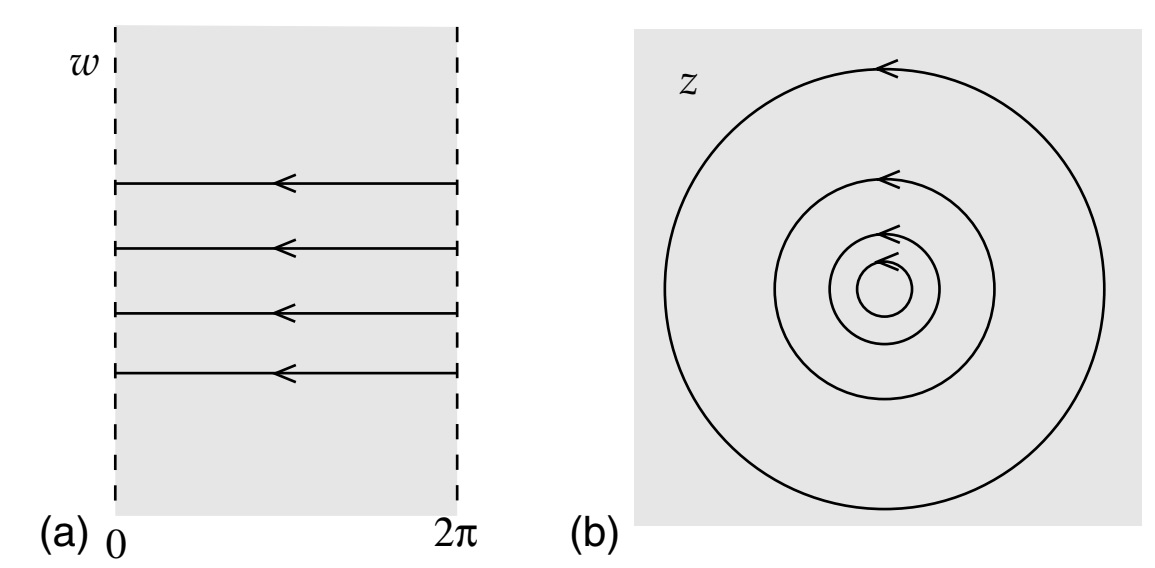
\includegraphics[width=0.8\textwidth,natwidth=866,natheight=426]{Fig2.3.jpg}\\
	\caption{Closed String Coordinates}
\end{center}
\end{figure}

在$w$坐标中, 时间对应于$\sigma^{2}=\operatorname{Im} w$ 的移动. 在z坐标中, 时间径向移动, 原点是遥远的过去. 这些坐标通过一个共形变换相关. 对于理论的正则解释, $w$坐标是自然的, 但$z$坐标也相当有用, 并且大多数表达式都写在这个参考系中.

对于全纯或反全纯算符, 我们可以做Laurent展开
\begin{equation}
T_{z z}(z)=\sum_{m=-\infty}^{\infty} \frac{L_{m}}{z^{m+2}}, \quad \tilde{T}_{\bar{z} \bar{z}}(\bar{z})=\sum_{m=-\infty}^{\infty} \frac{\tilde{L}_{m}}{\bar{z}^{m+2}} \label{2.6.5}
\end{equation}
展开系数称为Virasoro生成元. 由围道积分给出
\begin{equation}\label{2.6.6}
L_{m}=\oint_{C} \frac{\dif z}{2 \pi \mi z} \: z^{m+2} T_{z z}(z)
\end{equation}
其中C以逆时针围绕原点的任意围道. 在$\sigma^2=0$时, Laurent展开就是一个普通的Fourier变换
\begin{subequations} \label{2.6.7}
\begin{align}
T_{w w}(w)&=-\sum_{m=-\infty}^{\infty} \exp (\mi m \sigma^{1}-m \sigma^{2}) T_{m}   \label{2.6.7a}\\
T_{\bar{w} \bar{w}}(\bar{w})&=-\sum_{m=-\infty}^{\infty} \exp (-\mi m \sigma^{1}-m \sigma^{2}) \tilde{T}_{m} \label{2.6.7b}
\end{align}
\end{subequations}
其中
\begin{equation}\label{2.6.8}
T_{m}=L_{m}-\delta_{m, 0} \frac{c}{24} \:, \qquad \tilde{T}_{m}=\tilde{L}_{m}-\delta_{m, 0} \frac{\tilde{c}}{24} \:.
\end{equation}
$T_0$的额外偏移源于非张量变换(\ref{2.4.26})
\begin{equation}
T_{w w}=(\partial_{w} z)^{2} T_{z z}+\frac{c}{24} \:.
\end{equation}
在$w=\sigma^{1}+\mi \sigma^{2}$系中, 时间平移的哈密顿量是
\begin{equation}\label{2.6.10}
H=\int_{0}^{2 \pi} \frac{\dif \sigma^{1}}{2 \pi} \: T_{22}=L_{0}+\tilde{L}_{0}-\frac{c+\tilde{c}}{24} \:.
\end{equation}
注意Laurent展开中的+2, 它们在Fourier变换中被$T$的共形变换抵消. 类似地, 一个权重$h$的全纯场的Laurent展开将在指数上包含$h$.

将时间$\operatorname{Im} w=\ln |z|$为常数的圆上的路径积分剪开. Virasoro生成元变成通常意义上的算符. 由于全纯性, 积分(\ref{2.6.6})独立于$C$, 因而特别地, 在时间平移下不变. 即它们是守恒荷, 与共形不变相联系的荷. 

\begin{figure}[h]
	\begin{center}
		%	\includegraphics[width=0.8\textwidth,bb=0 0 1299 596]{Fig2.3ClosedStringCoordinates.jpg}\\
		%1px=0.75pt
		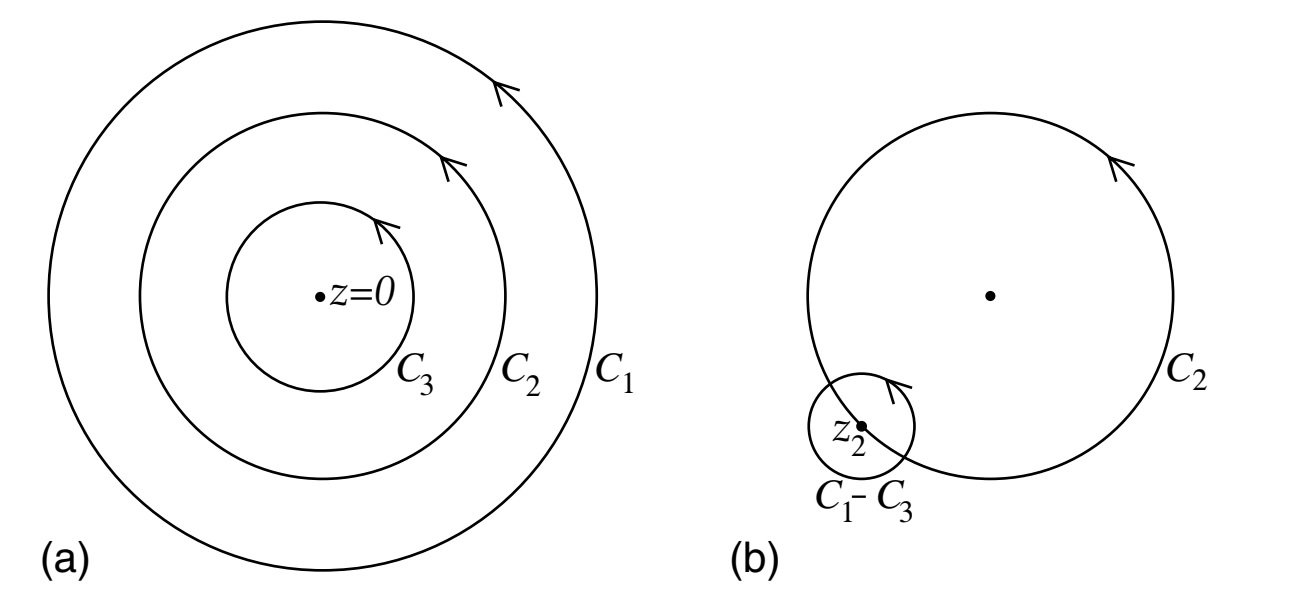
\includegraphics[width=0.6\textwidth,natwidth=974,natheight=447]{Fig2.4.jpg}\\
		\caption{围道}\label{Fig2.4}
	\end{center}
\end{figure}
一个重要的事实:流的OPE决定了对应荷的代数. 考察一般荷$Q_{i}, i=1,2$, 给定为全纯流的围道积分
\begin{equation}
Q_{i}\{C\}=\oint_{C} \frac{\dif z}{2 \pi \mi} j_{i}
\end{equation}
考察组合
\begin{equation}\label{2.6.12}
Q_{1}\{C_{1}\} Q_{2}\{C_{2}\}-Q_{1}\{C_{3}\} Q_{2}\{C_{2}\}
\end{equation}
围道如图\ref{Fig2.4}a所示.


因子写成的序列是无关的, 因为它们仅是一个路径积分中的积分变量(除非两个荷是反对易的. 在这种情况下会有一个额外的符号并且所有的对易子都会变成反对易子. 
当我们劈开路径积分以做一个算符解释. 决定算符序列的是时间顺序, 在这里是$t_{1}>t_{2}>t_{3}$. 对组合(\ref{2.6.12})的路径积分对应矩阵元
\begin{equation}
\hat{Q}_{1} \hat{Q}_{2}-\hat{Q}_{2} \hat{Q}_{1} \equiv [\hat{Q}_{1}, \hat{Q}_{2}]
\end{equation}
现在, 对于围道$C_2$上的一给定点$z_2$, 我们可以将$C_1, C_3$围道的差异进行变形, 如图\ref{Fig2.4}b所示, 所以对易子由OPE的留数给出
\begin{equation}
[Q_{1}, Q_{2}]\{C_{2}\}=\oint_{C_{2}} \frac{\dif z_{2}}{2 \pi \mi} \: \operatorname{Res}_{z_{1} \to z_{2}} j_{1}(z_{1}) j_{2}(z_{2}) \label{2.6.14}
\end{equation}
围道讨论允许我们在OPE与对易关系之间来回传递. 我们来强调一下, 对于守恒流, 知道了OPE中的奇异性等效于知道了对应荷的对易子代数. 将守恒荷$Q_{2}\left\{C_{2}\right\}$ 替换成任意算符, 上面的讨论同样适用:
\begin{equation}
[Q, \mathscr{A}(z_{2}, \bar{z}_{2})]=\operatorname{Res}_{z_{1} \to z_{2}} j(z_{1}) \mathscr{A}(z_{2}, \bar{z}_{2})
=\frac{1}{\mi \epsilon} \delta \mathscr{A}(z_{2}, \bar{z}_{2}) \label{2.6.15}
\end{equation}
这正是熟悉的陈述:荷$Q$生成了相对应的变换. 类似地, 对于反全纯流的围道积分
\begin{equation}
\tilde{Q}\{C\}=-\oint_{C} \frac{\dif \bar{z}}{2 \pi \mi} \: \tilde{\jmath} \:, \label{2.6.16}
\end{equation}
Ward 恒等式与围道讨论暗示了
\begin{equation}
[\tilde{Q}, \mathscr{A}(z_{2}, \bar{z}_{2})]=\operatorname{Res}_{\bar{z}_{1} \to \bar{z}_{2}} \tilde{\jmath}(\bar{z}_{1}) 
\mathscr{A}(z_{2}, \bar{z}_{2})=\frac{1}{\mi \epsilon} \delta \mathscr{A}(z_{2}, \bar{z}_{2}) \label{2.6.17}
\end{equation}
将其应用于Virasoro代数(\ref{2.6.6}), 
\begin{align}
&\operatorname{Res}_{z_{1} \to z_{2}} z_{1}^{m+1} T(z_{1}) z_{2}^{n+1} T(z_{2})  \nonumber \\
&\quad =\operatorname{Res}_{z_{1} \rightarrow z_{2}} z_{1}^{m+1} z_{2}^{n+1}\Biggl(\frac{c}{2 z_{12}^{4}}+\frac{2}{z_{12}^{2}} T(z_{2})
+\frac{1}{z_{12}} \partial T(z_{2})\Biggr) \nonumber \\
&\quad =\frac{c}{12}(\partial^{3} z_{2}^{m+1}) z_{2}^{n+1}+2(\partial z_{2}^{m+1}) z_{2}^{n+1} T(z_{2})
+z_{2}^{m+n+2} \partial T(z_{2}) \nonumber \\
&\quad =\frac{c}{12}(m^{3}-m) z_{2}^{m+n-1}+(m-n) z_{2}^{m+n+1} T(z_{2})+\text {全导数}  \label{2.6.18}
\end{align}
其中$j_{m}(z)=z^{m+1} T(z)$.
那么右边的$z_2$围道积分给出Virasoro代数:
\begin{equation}\label{2.6.19}
\left[L_{m}, L_{n}\right]=(m-n) L_{m+n}+\frac{c}{12}\left(m^{3}-m\right) \delta_{m,-n}
\end{equation}
$\tilde{L}_{m}$满足中心荷为$\tilde{c}$ 的相同代数.
因而任何CFT有无限个守恒荷, 即Virasoro生成元. 其作用在Hilbert空间中并满足代数(\ref{2.6.19}). 先关注几个简单的性质. 一般地, 处理$L_{0}$ 和 $\tilde{L}_{0}$ 的本征态, 生成元$L_{0}$ 满足
\begin{equation}
\left[L_{0}, L_{n}\right]=-n L_{n}
\end{equation}
如果$|\psi\rangle$ 是 $L_{0}$的本征值为h的本征态, 那么
\begin{equation}
L_{0} L_{n}|\psi\rangle=L_{n}\left(L_{0}-n\right)|\psi\rangle=(h-n) L_{n}|\psi\rangle
\end{equation}
所以$L_n|\psi\rangle$ 是本征值为$h-n$的本征态, $n<0$的生成元提高$L_{0}$的本征值, 而$n>0$则降低它.

三个生成元$L_{0}$ ,  $L_{\pm 1}$构成没有中心荷的闭代数:
\begin{equation}
\left[L_{0}, L_{1}\right]=-L_{1}, \quad\left[L_{0}, L_{-1}\right]=L_{-1}, \quad\left[L_{1}, L_{-1}\right]=2 L_{0}
\end{equation}
这是代数$SL(2,\mathds{R})$, 与$SU(2)$相差一个符号. 对于权重$(h,0)$的全纯张量场$\mathcal{O}$的Laurent系数
\begin{equation}
\mathcal{O}(z)=\sum_{m=-\infty}^{\infty} \frac{\mathcal{O}_{m}}{z^{m+h}} \label{2.6.23}
\end{equation}
从OPE \eqref{2.4.16}得到对易子
\begin{equation}
[L_{m}, \mathcal{O}_{n}]=[(h-1) m-n] \mathcal{O}_{m+n} \:. \label{2.6.24}
\end{equation}
又一次,  $n>0$的模减小$L_0$, $n<0$的模增大$L_0$.

\begin{tcolorbox}
\eqref{2.6.24}的证明: 在\eqref{2.6.17}中令$j_{m}(z)=z^{m+1} T(z)$以及$j_{n}(z)=z^{n+h-1} \mathcal{O}(z)$, 那么
\begin{align*}
&\quad \operatorname{Res}_{z_1 \rightarrow z_2}  z_1^{m+1} T(z_{1}) z_2^{n+h-1} \mathcal{O}(z_{2})\\
&=\operatorname{Res}_{z_1 \rightarrow z_2} z_1^{m+1} z_2^{n+h-1}\left(\frac{h}{z_{12}^2} O(z_2)+\frac{1}{z_{12}} \partial \mathcal{O}(z_2)\right)\\
&=h(\partial z_2^{m+1})z_2^{n+h-1}\mathcal{O}(z_2)+z_2^{m+n+h}\partial\mathcal{O}(z_2)\\
&=h(m+1)z_2^{m+n+h-1}\mathcal{O}(z_2)-(m+n+h)z_2^{m+n+h-1}\mathcal{O}(z_2)+ \text{全导数}
\end{align*}
利用\eqref{2.6.23}, 第一项变成
$$h(m+1)z_2^{m+n+h-1}\mathcal{O}(z_2) \sim h(m+1) \sum \mathcal{O}_q z_2^{m+n-q-1} \sim h(m+1)\mathcal{O}_{m+n}$$
第二项变成
\begin{align*}
-(m+n+h) z_{2}^{m+n+h-1} \sum \frac{\mathcal{O}_{q}}{z_{2}^{q+h}} \sim-(m+n+h) \mathcal{O}_{m+n}
\end{align*}
二者相加得\eqref{2.6.24}.
\end{tcolorbox}

在开弦中, 令
\begin{equation}
0 \leq \operatorname{Re} w \leq \pi \quad \Leftrightarrow \quad \operatorname{Im} z \geq 0
\end{equation}
其中
$z=-\exp (-\mi w)$. 
坐标区域如图\ref{Fig2.5}.
\begin{figure}[h]
	\begin{center}
		%	\includegraphics[width=0.8\textwidth,bb=0 0 778 341]{Fig2.3ClosedStringCoordinates.jpg}\\
		%1px=0.75pt
		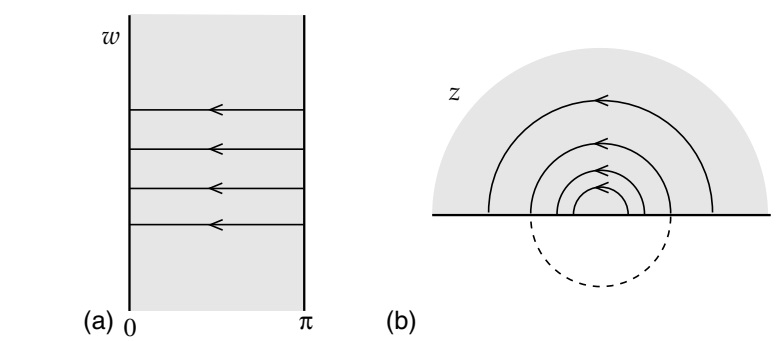
\includegraphics[width=0.8\textwidth,natwidth=584,natheight=256]{Fig2.5.jpg}\\
		\caption{Contours}\label{Fig2.5}
	\end{center}
\end{figure}


\noindent 在边界上, 能动量满足
\begin{equation}\label{2.6.26}
T_{a b} n^{a} t^{b}=0 \:,
\end{equation}
其中$n^{a}$和$t^{b}$分别是法向矢量和切向矢量. 为了看到这点, 考察边界是直线的坐标系. 边界的出现破坏了法向的平移不变性, 但不破坏切向, 使得流$T_{a b} t^{b}$ 依旧是守恒的. 那么边界条件(\ref{2.6.26})就是陈述流出边界的流是零. 在目前的情况下, 这变成
\begin{equation}
T_{w w}=T_{\bar{w} \bar{w}}, \: \operatorname{Re} w=0 \:, \pi \qquad \Leftrightarrow \quad T_{z z}=T_{\bar{z} \bar{z}}\:, \operatorname{Im} z=0 \:.
\end{equation}
使用“镜像法”(doubling trick)是方便的. 将下半$z$平面中的$T_{zz}$定义为$T_{\bar{z} \bar{z}}$在上半平面的镜像点$z^{\prime}=\bar{z}$处的值:
\begin{equation}
T_{z z}(z) \equiv T_{\bar{z} \bar{z}}\left(\bar{z}^{\prime}\right), \quad \operatorname{Im} z<0 \:.
\end{equation}
运动方程与边界条件总结为:$T_{z z}$在整个复平面全纯. 因为边界条件耦合了$T$ 和 $\widetilde{T}$, 所以仅存在一组 Virasoro 代数:
\begin{align}
L_{m} &=\frac{1}{2 \pi \mi} \int_{C}\Bigl(\dif z \:z^{m+1} T_{z z}-\dif \bar{z} \: \bar{z}^{m+1} T_{\bar{z} \bar{z}}\Bigr) \nonumber  \\
&=\frac{1}{2 \pi \mi} \oint \dif z\: z^{m+1} T_{z z}(z)
\end{align}
第一行中, 围道是中心为原点的半圆;第二行, 我们使用了“镜像法”(doubling trick)将$L_m$写成了闭合围道. 又一次, 这些$L_{m}$满足 Virasoro 代数
\begin{equation}
\left[L_{m}, L_{n}\right]=(m-n) L_{m+n}+\frac{c}{12}\left(m^{3}-m\right) \delta_{m,-n} \:.
\end{equation}

\section{\texorpdfstring{模式展开}{2.7 Mode expansions}} \label{sec:2.7}

\subsection*{自由标量}
在自由场论中, 场分解成谐振子, 并且频谱与能动量张量可以以模的形式上
给出. 我们从闭弦开始. 在$X^\mu$的理论中,  $\partial X$ 和 $\bar{\partial} X$是反全纯的. 所以有类似的Laurent展开:
\begin{equation}\label{2.7.1}
\partial X^{\mu}(z)=-\mi\biggl(\frac{\alpha^{\prime}}{2}\biggr)^{1 / 2} \sum_{m=-\infty}^{\infty} \frac{\alpha_{m}^{\mu}}{z^{m+1}}\:, \qquad 
\bar{\partial} X^{\mu}(\bar{z})=-\mi\biggl(\frac{\alpha^{\prime}}{2}\biggr)^{1 / 2} \sum_{m=-\infty}^{\infty} \frac{\tilde{\alpha}_{m}^{\mu}}{\bar{z}^{m+1}} \:.
\end{equation}
等效地, 
\begin{subequations}\label{2.7.2}
\begin{align}
\alpha_{m}^{\mu}&=\biggl(\frac{2}{\alpha^{\prime}}\biggr)^{1 / 2} \oint \frac{\dif z}{2 \pi}\: z^{m} \partial X^{\mu}(z) \:, \label{2.7.2a} \\
\tilde{\alpha}_{m}^{\mu}&=-\biggl(\frac{2}{\alpha^{\prime}}\biggr)^{1 / 2} \oint \frac{\dif \bar{z}}{2 \pi} \: \bar{z}^{m} \bar{\partial} X^{\mu}(\bar{z}) \:. \label{2.7.2b}
\end{align}
\end{subequations}
$X^\mu$的单值性暗示着$\alpha_{0}^{\mu}=\tilde{\alpha}_{0}^{\mu}$, 更进一步, 时空平移的Noether流是$\mi \partial_{a} X^{\mu} / \alpha^{\prime}$, 
所以时空动量
\begin{equation}\label{2.7.3}
p^{\mu}=\frac{1}{2 \pi \mi} \oint_{C} (\dif z \: j^{\mu}-\dif \bar{z}\: \tilde{\jmath}^{\mu})
=\biggl(\frac{2}{\alpha^{\prime}}\biggr)^{1 / 2} \alpha_{0}^{\mu}=\biggl(\frac{2}{\alpha^{\prime}}\biggr)^{1 / 2} \tilde{\alpha}_{0}^{\mu}
\end{equation}
对表达式(\ref{2.7.1}) 积分给出
\begin{equation}
X^{\mu}(z, \bar{z})=x^{\mu}- \mi \frac{\alpha^{\prime}}{2} p^{\mu} \ln |z|^{2}+\mi\left(\frac{\alpha^{\prime}}{2}\right)^{1 / 2} \sum_{\substack{m=-\infty  \\  m \neq 0}}^{\infty} \frac{1}{m}\left(\frac{\alpha_{m}^{\mu}}{z^{m}}+\frac{\tilde{\alpha}_{m}^{\mu}}{\bar{z}^{m}}\right) \:.
\end{equation}
无论是从标准正则对易出发, 还是从围道讨论或者$XX$ OPE, 可以给出
\begin{subequations} \label{2.7.5}
\begin{align}
[\alpha_{m}^{\mu}, \alpha_{n}^{\nu}] &= [\tilde{\alpha}_{m}^{\mu}, \tilde{\alpha}_{n}^{\nu}]=m \delta_{m,-n} \eta^{\mu \nu} \:, \label{2.7.5a} \\
[x^{\mu}, p^{\nu}] &= \mi \eta^{\mu \nu} \:, \label{2.7.5b}  
\end{align}
\end{subequations}
其他对易子为零. 频谱从动量为$k^\mu$的态$\lvert 0 ; k\rangle$ 开始, 这个态被所有$n>0$的下降模$\alpha_n^\mu$湮灭, 而频谱中的其它态由上升模$(n<0)$以所有可能的方式作用在$\lvert 0 ; k\rangle$给出. 

我们现在希望以模算符的形式展开 Virasoro 生成元. 将$X^\mu$ 的 Laurent 展开式代入能动量张量(\ref{2.4.4}) 并对$z$的给定阶合并同类项, 给出
\begin{equation}\label{2.7.6}
L_{m} \sim \frac{1}{2} \sum_{n=-\infty}^{\infty} \alpha_{m-n}^{\mu} \alpha_{\mu n} \:.
\end{equation}
``$\sim$''是指忽略了算符的顺序. 当$m\neq 0$时 , 展开式\eqref{2.7.6}是定义良好的且正确的——每一项的模算符对易所以序列不重要. 对于$m=0$, 
将下降算符放在右边并引入正规编序常数,
\begin{equation}
 	L_{0}=\frac{\alpha^{\prime} p^{2}}{4}+\sum_{n=1}^{\infty}\left(\alpha_{-n}^{\mu} \alpha_{\mu n}\right)+a^{X} \:. \label{2.7.7}
\end{equation}
我们在\ref{sec:1.3}节中遇到了同一问题, 在那里我们以一种启发式的方法处理. 现在左边一个有限且明确的定义, 用$\mathrel{:\::}$-编序的能动量张量中的Laurent系数进行定义, 所以规范序列常数是有限且可计算的. 有几种方式可以决定它, 最简单的是用 Virasoro 代数,
 \begin{equation}\label{2.7.8}
 2 L_{0}|0 ; 0\rangle=(L_{1} L_{-1}-L_{-1} L_{1})|0 ; 0\rangle=0  \:,
 \end{equation}
因而
 \begin{equation}
 a^{X}=0 \:. \label{2.7.9}
 \end{equation}
这里我们使用了$L_1, L_{-1}$ 的已知形式: 每一项要么包含下降算符, 要么包含$p^\mu$, 因而湮灭了$|0 ; 0\rangle$. 

从 OPE 中, 我们决定了 Virasoro 代数的中心荷. 它也可以从 Virasoro 代数的模算符表达式直接得出.

引入一个新的记法. 符号$ \mathrel{\typecolon \:\typecolon}$ 代表产生-湮灭正规编序: 将所有下降算符放在所有产生算符右边. 注意交换反对易算符时有一个负号. 
由于这个原因, 我们将$p^\mu$纳入下降算符, 将$x^\mu$纳入上升算符. 在这个记号下, 我么可以写
\begin{equation}\label{2.7.10}
L_{m}=\frac{1}{2} \sum_{n=-\infty}^{\infty}\mathrel{ \typecolon\alpha_{m-n}^{\mu} \alpha_{\mu n}\typecolon}
\end{equation}


我们现在引入了两种正规序列形式, 即共形正规序列$\mathrel{:\::}$与产生-湮灭正规序列$\mathrel{\typecolon\:\typecolon}$. 前者的优势是, 它所产生的算符, 其 OPE 与共形变换性质较为简单; 后者对于读者可能更为熟悉, 它在处理算符的矩阵元时比较方便. 我们现在要给出二者关系. 从比较编时乘积与产生-湮灭正规乘积开始. 对于 $\lvert z \rvert >\lvert z^{\prime}\rvert$的乘积$X^{\mu}(z, \bar{z}) X^{\nu}(z^{\prime}, \bar{z}^{\prime})$, 代入模展开, 并将$X^{\mu}(z, \bar{z})$ 中的下降算符挪到右边:
\begin{align}
X^{\mu}(z, \bar{z}) X^{\nu}(z^{\prime}, \bar{z}^{\prime}) &=  \mathrel{\typecolon X^{\mu}(z, \bar{z}) X^{\nu}(z^{\prime}, \bar{z}^{\prime}) \typecolon}  \nonumber \\
&\qquad \qquad +\frac{\alpha^{\prime}}{2} \eta^{\mu \nu}\left[-\ln |z|^{2}+\sum_{m=1}^{\infty} \frac{1}{m}\left(\frac{z^{\prime m}}{z^{m}}+\frac{\bar{z}^{\prime m}}{\bar{z}^{m}}\right)\right] \nonumber \\
&=\mathrel{\typecolon X^{\mu}(z, \bar{z}) X^{\nu}(z^{\prime}, \bar{z}^{\prime}) \typecolon}-\frac{\alpha^{\prime}}{2} \eta^{\mu \nu}\ln \lvert z-z^\prime\rvert^{2} \label{2.7.11}
\end{align}
由于$|z|>\lvert z^{\prime}\rvert$, 左边是编时的且求和收敛. 定义\eqref{2.1.21}给出的编时乘积与共形正规乘积的关系(定义\eqref{2.1.21}用的是路径积分的语言, 所以右边的乘积在算符体系下是编时的). 这与\eqref{2.7.11}是相同的, 使得
\begin{equation}\label{2.7.12}
\mathrel{\typecolon X^{\mu}(z, \bar{z}) X^{\nu}(z^{\prime}, \bar{z}^{\prime})\typecolon} = \mathrel{: X^{\mu}(z, \bar{z}) X^{\nu}(z^{\prime}, \bar{z}^{\prime})}:
\end{equation}
这种关系在一般的 CFT 中并不成立, 并且实际上, $p^\mu$与下降算符的某些组合给出更简单的结果. 对于算符的$w$形式的共形正规序列这也不成立.
从(\ref{2.7.12})可以立即写出模展开(\ref{2.7.10}), 并给出$a^{X}=0$的第二种推导.

超过两个$X^\mu$的产生-湮灭正规乘积与$\mathrel{:\::}$编序有相同的组合学因子. 即, 它们都是从编时乘积中通过对所有的收缩求和获得的——场论中的 Wick 定理. 
为了将算符的正规序从一种形式转化到另一种形式, 用两点函数之差进行收缩并求和. 即, 如果我们有两种序,
\begin{equation}
[X^{\mu}(z, \bar{z}) X^{v}(z^{\prime}, \bar{z}^{\prime})]_{1} = [X^{\mu}(z, \bar{z}) X^{v}(z^{\prime}, \bar{z}^{\prime})]_{2} 
+\eta^{\mu v} \Delta (z, \bar{z}, z^{\prime}, \bar{z}^{\prime}) \:, \label{2.7.13}
\end{equation}
那么对于一般算符$\mathscr{F}$
\begin{equation}
[\mathscr{F}]_{1}=\exp \left(\frac{1}{2} \int \dif^{2} z\, \dif^{2} z^{\prime}\: \Delta(z, \bar{z}, z^{\prime}, \bar{z}^{\prime}) \frac{\delta}{\delta X^{\mu}(z, \bar{z})} \frac{\delta}{\delta X_{\mu}(z^{\prime}, \bar{z}^{\prime})}\right)[\mathscr{F}]_{2} \:. \label{2.7.14}
\end{equation}

对于线性伸缩子 CFT, Laurent 展开与对易子不变, 而 Virasoro 生成元包含一个额外项
\begin{equation}
L_{m}=\frac{1}{2} \sum_{n=-\infty}^{\infty} \mathrel{\typecolon \alpha_{m-n}^{\mu} \alpha_{\mu n}\typecolon} + \:\mi\left(\frac{\alpha^{\prime}}{2}\right)^{1 / 2}(m+1) V^{\mu} \alpha_{\mu m} \:.
\end{equation}

\subsection*{ $bc$ CFT}

场$b$和$c$有Laurent展开
\begin{equation} \label{2.7.16}
b(z)=\sum_{m=-\infty}^{\infty} \frac{b_{m}}{z^{m+\lambda}}\:, \qquad c(z)=\sum_{m=-\infty}^{\infty} \frac{c_{m}}{z^{m+1-\lambda}} \:.
\end{equation}
精确些, 如果$\lambda$是整数, 它们仅是 Laurent 展开. 半整数的情况也是有趣的, 我们将在第10章细致地处理它. OPE 给出反对易子
\begin{equation}
\left\{b_{m}, c_{n}\right\}=\delta_{m,-n} \:. \label{2.7.17}
\end{equation}
首先考察被所有$n>0$的算符消灭的态. $b_0$和$c_0$的振子代数生成两个这样的基态$\lvert\downarrow\rangle$ 和 $\lvert\uparrow\rangle$. 其有性质
\begin{subequations} \label{2.7.18}
\begin{align}
b_{0}\lvert\downarrow\rangle &=0\:, \quad b_{0} \lvert \uparrow\rangle=\lvert\downarrow\rangle \:, \label{2.7.18a} \\
c_{0}\lvert\downarrow\rangle &=\lvert\uparrow\rangle \:, \quad c_{0}\lvert\uparrow\rangle=0 \:, \label{2.7.18b} \\
b_{n}\lvert\downarrow\rangle &=b_{n}\lvert\uparrow\rangle=c_{n}\lvert \downarrow\rangle=c_{n}\lvert\uparrow\rangle=0 \:, \quad n>0  \:. \label{2.7.18c}
\end{align}
\end{subequations}
普通的态通过用$n<0$的模作用这些态获得, 不过由于反对易, 最多作用一次. 由于之后的某些原因, 将$b_0$与下降算符组队, $c_0$与上升算符组队将是方便的, 所以我们挑出$\lvert \downarrow\rangle$ 作为鬼真空$|0\rangle$. 在弦论中我们将有一个全纯的$bc$理论和一个反全纯的$\tilde{b} \tilde{c}$ 理论. 每一个有$\lambda=2$. 
而闭弦频谱则包含两对理论的乘积.

Virasoro 生成元是
\begin{equation}
L_{m}=\sum_{n=-\infty}^{\infty}(m \lambda-n) \mathrel{\typecolon b_{n} c_{m-n}\typecolon}+ \:\delta_{m, 0} a^{\mathrm{g}} \:. \label{2.7.19}
\end{equation}
编序常数可以用(\ref{2.7.8})那样决定, 它给出
\begin{align}
2 L_{0}\lvert \downarrow\rangle &= (L_{1} L_{-1}-L_{-1} L_{1}) \lvert \downarrow\rangle \nonumber \\
&= (\lambda b_{0} c_{1})[(1-\lambda) b_{-1} c_{0}]\lvert \downarrow\rangle=\lambda(1-\lambda)\lvert \downarrow\rangle \:. \label{2.7.20}
\end{align}
因而$a^{\mathrm{g}}=\frac{1}{2} \lambda(1-\lambda)$并且
\begin{equation}
L_{m}=\sum_{n=-\infty}^{\infty}(m \lambda-n) \mathrel{\typecolon b_{n} c_{m-n}\typecolon} + \: \frac{\lambda(1-\lambda)}{2} \delta_{m, 0} \:.
\label{2.7.21}
\end{equation}
常数也可以通过解出$\mathrel{:\::}$和$\mathrel{\typecolon\:\typecolon}$的关系获得. 对于鬼数流\eqref{2.5.14}, $j={-}:\mathrel{bc}:$, 荷是
\begin{align}
N^{\mathrm{g}} &=-\frac{1}{2 \pi \mi} \int_{0}^{2 \pi} \dif w \: j_{w} \nonumber \\
&=\sum_{n=1}^{\infty}(c_{-n} b_{n}-b_{-n} c_{n})+c_{0} b_{0}-\frac{1}{2} \:. \label{2.7.22}
\end{align}
它满足
\begin{equation}
[N^{\mathrm{g}}, b_{m}]=-b_{m}\:, \qquad  [N^{\mathrm{g}}, c_{m}]=c_{m} \:, \label{2.7.23}
\end{equation}
因而$c$数减去$b$数是激发. 基态有鬼数$\pm \frac{1}{2}$:
\begin{equation}
N^{\mathrm{g}}\lvert \downarrow\rangle = -\frac{1}{2}\lvert \downarrow\rangle \:, \qquad 
N^{\mathrm{g}}\lvert \uparrow\rangle = \frac{1}{2}\lvert \uparrow\rangle \:. \label{2.7.24}
\end{equation}
这依赖于编序常数的值, 但可以进行猜测: 基态的平均鬼数应该是零且鬼数在$b \leftrightarrow c$ 下改变符号.

\subsection*{ 开弦}
在开弦中, Neumann边界条件变成了实轴上的$\partial_z X^{\mu}=\partial_{\bar{z}} X^{\mu}$.
仅存在一组模, 边界条件要求展开式(\ref{2.7.1})中$\alpha_{m}^{\mu}=\tilde{\alpha}_{m}^{\mu}$. 时空动量积分 (\ref{2.7.3})只积半圆, 所以现在的归一化是
\begin{equation}
\alpha_{0}^{\mu}= (2 \alpha^{\prime})^{1 / 2} p^{\mu} \:. \label{2.7.25}
\end{equation}
那么$X^\mu$的展开是
\begin{equation}
X^{\mu}(z, \bar{z})=x^{\mu}- \mi \alpha^{\prime} p^{\mu} \ln |z|^{2} + \mi\left(\frac{\alpha^{\prime}}{2}\right)^{1 / 2} 
\sum_{\substack{m=-\infty  \\  m \neq 0}}^{\infty} \frac{\alpha_{m}^{\mu}}{m} (z^{-m}+\bar{z}^{-m}) \:. \label{2.7.26}
\end{equation}
另外
\begin{equation}
L_{0}=\alpha^{\prime} p^{2}+\sum_{n=1}^{\infty} \alpha_{-n}^{\mu}\cdot \alpha_{\mu n} \:. \label{2.7.27}
\end{equation}
对易子像往常一样
\begin{equation}
[\alpha_{m}^{\mu}, \alpha_{n}^{\nu}]=m \delta_{m,-n} \eta^{\mu \nu} \: , \qquad [x^{\mu}, p^{\nu}]= \mi \eta^{\mu \nu} \:. \label{2.7.28}
\end{equation}

对于$bc$理论, 与弦相关的边界条件是
\begin{equation}
c(z)=\tilde{c}(\bar{z})\: , \quad b(z)=\tilde{b}(\bar{z}) \:, \quad \operatorname{Im} z=0 \:,  \label{2.7.29}
\end{equation}
这是$z$坐标的形式, 其中边界在实轴上. 那么我们可以用镜像法(doubling trick)将上半平面的全纯场和反全纯场写成整个平面中的全纯场的形式
\begin{equation}
c(z) \equiv \tilde{c}(\bar{z}^{\prime})\:, \quad b(z) \equiv \tilde{b}(\bar{z}^{\prime})\:, \quad \operatorname{Im}(z) \leq 0\,,\: z^{\prime}=\bar{ z} \:.  \label{2.7.30}
\end{equation}
因此对于开弦, 每个$b$和$c$有一组Laurent展开.

\section{\texorpdfstring{顶点算符}{2.8 Vertex operators}}

在量子场论中, 一方面, 既有理论的态空间; 另一方面, 又有定域算符的集合. 在共形场论中, 当在圆上量子化CFT时, 它们之间有一个简单且有用的同构. 考察$w$-坐标中的半无限大圆柱,
\begin{equation}
0 \leq \operatorname{Re} w \leq 2 \pi \:, \quad w \sim w+2 \pi \:, \quad \operatorname{Im} w \leq 0 \:, \label{2.8.1}
\end{equation}
在$z=\exp (-\mi w)$下, 这个半无限大圆柱被映射到一个单位圆盘. 如图\ref{Fig2.6}所示.
\vspace*{-2cm}
\begin{figure}[h]
\begin{center}
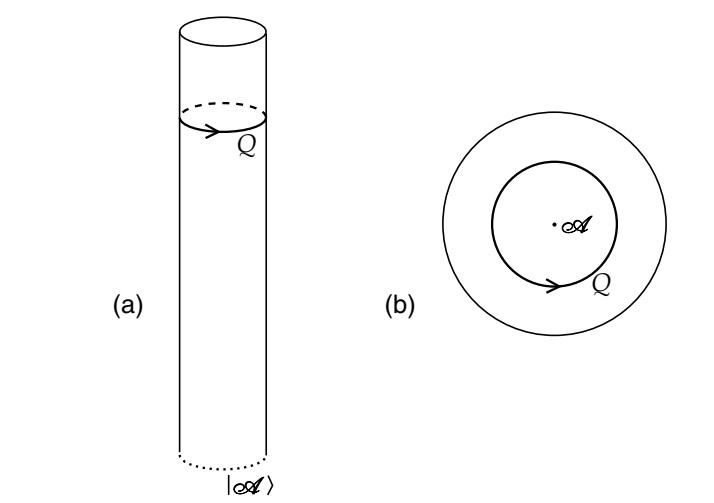
\includegraphics[width=0.8\textwidth,natwidth=535,natheight=377]{Fig2.6.jpg}
\caption{(a) $w$-坐标下的半无限大圆柱, 带有初态$\lvert\mathscr{A}\rangle$ 和荷$Q$. 
(b)共形等价单位圆盘, 带有定域算符$\mathscr{A}$和$Q$的围道积分.}\label{Fig2.6}
\end{center}
\end{figure}

对于自由场论, 容易得到这个同构的详细形式. 假定有一守恒荷$Q$以图 \ref{Fig2.6}(a) 那样的方式作用在态$\lvert\mathscr{A}\rangle$ 上. 通过使用 OPE 计算图 \ref{Fig2.6}(b) 中的围道积分, 可以发现对应的定域算符. 对应于单位算符, 我们等同态$|1\rangle$. 在原点没有算符时, $\partial X^{\mu}$ 和 $\bar{\partial} X^{\mu}$在图\ref{Fig2.6}(b) 中$Q$的围道内是全纯和反全纯的. 定义$m \geq 0$ 的$\alpha_{m}^{\mu}$ 和 $\tilde{\alpha}_{m}^{\mu}$的围道积分(\ref{2.7.2})没有极点, 所以给出零. $\lvert 1\rangle$ 被这些模消灭, 这表明它是基态,
\begin{equation}
\lvert 1\rangle=\lvert 0 ; 0\rangle \:, \label{2.8.2}
\end{equation}
现在考察, 例如$m$为正的态$\alpha_{-m}^{\mu}|1\rangle$. 过渡到图 \ref{Fig2.6}(b), $Q=\alpha_{-m}^{\mu}$, 场在围道内是全纯的, 因此对于$m\geq 1$得到
\begin{equation}\label{2.8.3}
\alpha_{-m}^{\mu}=\left(\frac{2}{\alpha^{\prime}}\right)^{1 / 2} \oint \frac{\dif z}{2 \pi} \: z^{-m} \partial X^{\mu}(z) \rightarrow\left(\frac{2}{\alpha^{\prime}}\right)^{1 / 2} \frac{\mi}{(m-1) !} \partial^{m} X^{\mu}(0)
\end{equation}
所以
\begin{equation}
\alpha_{-m}^{\mu}\lvert 1\rangle \cong\left(\frac{2}{\alpha^{\prime}}\right)^{1 / 2} \frac{\mi}{(m-1) !} \partial^{m} X^{\mu}(0)\:, \quad m \geq 1 \:. \label{2.8.4}
\end{equation}
类似地
\begin{equation}
\tilde{\alpha}_{-m}^{\mu}|1\rangle \cong\left(\frac{2}{\alpha^{\prime}}\right)^{1 / 2} \frac{\mi}{(m-1) !} \bar{\partial}^{m} X^{\mu}(0)\:, \quad m \geq 1 \:. \label{2.8.5}
\end{equation}
当$\alpha_{-m}^{\mu}$ 或 $\tilde{\alpha}_{-m}^{\mu}$ 作用在一般态$|\mathscr{A}\rangle$上时, 这个对应依旧成立. 如果$:\mathrel{ \mathscr{A}(0,0)}:$ 是任意的正规编序算符, 在$\partial X^{\mu}(z)$ 与 $:\mathrel{ \mathscr{A}(0,0)}:$ 的算符乘积中可能会有奇异性, 
但不难对$m>0$验证
\begin{equation}
\alpha_{-m}^{\mu} :\mathrel{\mathscr{A}(0,0)}:=:\mathrel{ \alpha_{-m}^{\mu} \mathscr{A}(0,0)}:  \:. \label{2.8.6}
\end{equation}
这是因为该收缩的围道积分将不可能有单奇点, 那么可以在正规序列中进行相同的运算(\ref{2.8.3}), 因而有数个$\alpha$振子激发的态作为相对应算符的$\mathrel{:\::}$正规乘积出现
\begin{subequations}\label{2.8.7}
\begin{align}
\alpha_{-m}^{\mu} &\rightarrow \mi\left(\frac{2}{\alpha^{\prime}}\right)^{1 / 2} \frac{1}{(m-1) !} \partial^{m} X^{\mu}(0)\:, \quad m \geq 1 \:,  \\
\tilde{\alpha}_{-m}^{\mu} &\rightarrow \mi\left(\frac{2}{\alpha^{\prime}}\right)^{1 / 2} \frac{1}{(m-1) !} \bar{\partial}^{m} X^{\mu}(0)\:, \quad m \geq 1 \:,
\end{align}
\end{subequations}
类似地
\begin{equation}\label{2.8.8}
x_{0}^{\mu} \rightarrow X^{\mu}(0,0) \:.
\end{equation}
通过用(\ref{2.8.7}) 和(\ref{2.8.8}) 左边的算符作用在$|1\rangle$ 上可以获得任何算符. 
对应该态的算符就由右边相对应的定域算符的$\mathrel{:\::}$正规乘积给定. 例如,
\begin{equation}
\lvert 0 ; k\rangle \cong \: : \mathrel{\me^{\mi k \cdot X(0,0)}}: \:. \label{2.8.9}
\end{equation}
这很容易理解: 在平移$X^{\mu} \rightarrow X^{\mu}+a^{\mu}$ 下, 态与相对应算符有相同的平移, 均乘以$\me ^{\mi k\cdot a}$. 

同一方法适用于$bc$理论. 明晰起见, 我们指定$\lambda=2$的情况. 这是玻色弦论感兴趣的. 从 Laurent 展开与围道讨论给出
\begin{equation}\label{2.8.10}
b_{m}|1\rangle=0, \quad m \geq-1, \qquad c_{m}|1\rangle=0, \quad m \geq 2 \:.
\end{equation}
注意 Laurent 展开指数中的偏移, 它源于$b$和$c$的共形权重. 单位算符不再映射到基态上. 反而, 关系\eqref{2.8.10}决定了
\begin{equation}
\lvert 1\rangle=b_{-1}\lvert \downarrow\rangle \:. \label{2.8.11}
\end{equation}
上升算符的翻译是直接的,
\begin{subequations} \label{2.8.12}
\begin{align}
b_{-m} &\rightarrow \frac{1}{(m-2) !} \partial^{m-2} b(0)\:, \quad m \geq 2 \:, \label{2.8.12a}  \\
c_{-m} &\rightarrow \frac{1}{(m+1) !} \partial^{m+1} c(0)\:, \quad m \geq-1 \:. \label{2.8.12b}
\end{align}
\end{subequations}
注意, 鬼数为$-\frac{3}{2}$的态$b_{-1}\lvert \downarrow\rangle$被映射到鬼数为0的单位算符, 而鬼数为$-\frac{1}{2}$的态$\lvert \downarrow\rangle$被映射到鬼数为1的算符$c$. 这一差异源于鬼数流的非张量性质\eqref{2.5.17},
\begin{equation}
(\partial_{z} w) j_{w}(w)=j_{z}(z)+q_{0} \frac{\partial_{z}^{2} w}{\partial_{z} w}=j_{z}(z)-\frac{q_{0}}{z} \:, \label{2.8.13}
\end{equation}
其中$q_{0}=\lambda-\frac{1}{2}=\frac{3}{2}$. 圆柱参考系表达式\eqref{2.7.22}通常定义了态的鬼数, 而图\ref{Fig2.6}的围道讨论将顶点算符的鬼数与极坐标系荷关系起来
\begin{equation}
Q^{\mathrm{g}} \equiv \frac{1}{2 \pi i} \oint \dif z\: j_{z}=N^{\mathrm{g}}+q_{0} \:.\label{2.8.14}
\end{equation}
这也适用于其他荷:对于张量流, 态与相对应算符的荷是相等的.

上面大多数讨论可扩张到$\beta\gamma$理论, 但在超弦下存在一定困难. 

本节所有概念可扩展至开弦. 半无限大带
\begin{equation}
0 \leq \operatorname{Re} w \leq \pi, \quad \operatorname{Im} w \leq 0 \:, \label{2.8.15}
\end{equation}
在$z=-\exp (-\mi w)$下被映射至一个半圆盘, 即上半平面与单位圆的交叠区域. 初态又一次映射至原点, 其在边界上, 所以存在同构
\begin{equation}
\text {边界上的定域算符 } \leftrightarrow \text {交界上的态} \:. \label{2.8.16}
\end{equation}
细节与之上相同. 镜像法(doubling trick)在围道讨论中是有用的.

\subsection*{路径积分推导}
考察$z$平面的一个圆盘, 在原点处有定域算符$\mathscr{A}$, 要做路径积分的场是$\phi$, 这个场在单位圆上取固定的边界值$\phi_{\mathrm{b}}$. 
对圆盘内部场$\phi_i$做路径积分的同时保持$\phi_{\mathrm{b}}$不变, 这给出了泛函$\Psi_{\mathscr{A}}[\phi_{\mathrm{b}}]$,
\begin{equation}
	\Psi_{\mathscr{A}}[\phi_{\mathrm{b}}]=\int[\dif  \phi_{\mathrm{i}}]_{\phi_{\mathrm{b}}} 
	\exp (-S[\phi_{\mathrm{i}}]) \mathscr{A}(0) \:. \label{2.8.17}
\end{equation}
场的泛函是态的 Schr\"{o}dinger 表示, 所以这是从算符到态的映射. Schr\"{o}dinger 表示为每个场构形赋予了一个复振幅, 有很多用途.

以另一种方式, 从某个态$\Psi[\phi_{\mathrm{b}}]$出发. 考察在圆环区域$1 \geq |z| \geq r$ 上的路径积分, 
其中保持外圆上的场$\phi_{\mathrm{b}}$固定, 而沿着内圆对$\phi_{\mathrm{b}}^\prime$ 作如下积分:
\begin{equation}\label{2.8.18}
\int [d \phi_{\mathrm{i}}]_{\phi_{\mathrm{b}}, \phi_{\mathrm{b}}^{\prime}} [\dif \phi_{\mathrm{b}}^{\prime}]\:
  \exp (-S[\phi_{\mathrm{i}}])\, r^{-L_{0}-\tilde{L}_{0}} \Psi[\phi_{\mathrm{b}}^{\prime}]
\end{equation}
即这个积分是在加权$r^{-L_{0}-\tilde{L}_{0}} \Psi[\phi_{\mathrm{b}}^{\prime}]$下进行的. 现在, 
对圆盘的路径积分恰好对应从 $|z|=r$到 $|z|=1$的传播, 其等价于用算符 $r^{+L_{0}+\tilde{L}_{0}}$作用. 这抵消了作用在$\Phi$上的算符, 所以\eqref{2.8.18}又一次是$\Psi[\phi_{\mathrm{b}}]$. 现在取$r\to 0$的极限. 圆环变成圆盘, 而对内圆的路径积分的极限可以认为是在原点处定义了某个定域算符. 根据这个构造, 圆盘上的路径积分与这个算符重新产生了边界上的$\Psi[\phi_{\mathrm{b}}]$. 

我们用一个自由标量场$X$来做例子. 在单位圆上展开
\begin{equation}
X_{\mathrm{b}}(\theta)=\sum_{n=-\infty}^{\infty} X_{n} \me^{\mi n \theta} \:, \quad X_{n}^{*}=X_{-n} \:. \label{2.8.19}
\end{equation}
边界态$\Psi[X_b]$可以认为是所有$X_n$的函数. 首先辨认出对应于单位算符的态, 它由没有插入任何算符的路径积分给出
\begin{equation}
\Psi_{1}[X_{\mathrm{b}}] = \int [\dif X_{\mathrm{i}}]_{X_{\mathrm{b}}} \exp \left(-\frac{1}{2 \pi \alpha^{\prime}} 
\int \dif^{2} z\: \partial X \bar{\partial} X\right) \:. \label{2.8.20}
\end{equation}
用通常的高斯法计算它. 将$X_i$分解成经典部分与涨落
\begin{subequations} \label{2.8.21}
\begin{align}
X_{\mathrm{i}}&=X_{\mathrm{cl}}+X_{\mathrm{i}}^{\prime} \:,\label{2.8.21a} \\
X_{\mathrm{cl}}(z, \bar{z})&=X_{0}+\sum_{n=1}^{\infty}\left(z^{n} X_{n}+\bar{z}^{n} X_{-n}\right)  \:. \label{2.8.21b}
\end{align}
\end{subequations}
在这个定义下, $X_{\text{cl}}$满足运动方程, $X_{\text{i}}^\prime$在边界上为零. 那么路径积分变成
\begin{equation}
\Psi_{1}[X_{\mathrm{b}}]=\exp (-S_{\mathrm{cl}}) \int [\dif X_{\mathrm{i}}^{\prime}]_{X_{\mathrm{b}}=0} 
\exp \left(-\frac{1}{2 \pi \alpha^{\prime}} \int \dif^{2} z\: \partial X^{\prime} \bar{\partial} X^{\prime}\right) \:,
\label{2.8.22}
\end{equation}
其中
\begin{align}
S_{\mathrm{cl}} &=\frac{1}{2 \pi \alpha^{\prime}} \sum_{m, n=1}^{\infty} m n X_{m} X_{-n} 
\int_{|z|<1} \dif^{2} z\: z^{m-1} \bar{z}^{n-1}  \nonumber \\
&=\frac{1}{\alpha^{\prime}} \sum_{m=1}^{\infty} m X_{m} X_{-m} \:. \label{2.8.23}
\end{align}
对$X_i^\prime$的积分是独立于边界条件的常数, 所以
\begin{equation}\label{2.8.24}
\Psi_{1}[X_{\mathrm{b}}] \propto \exp \left(-\frac{1}{\alpha^{\prime}} \sum_{m=1}^{\infty} m X_{m} X_{-m}\right) \:.
\end{equation}
这是高斯型, 实际上是基态. 为了看到这点, 在 Schr\"{o}dinger 基下写出上升下降算符,
\begin{subequations} \label{2.8.25}
\begin{align}
\alpha_{n}=-\frac{\mi n}{(2 \alpha^{\prime})^{1 / 2}} X_{-n}-\mi\left(\frac{\alpha^{\prime}}{2}\right)^{1 / 2} \frac{\partial}{\partial X_{n}} \:, \label{2.8.25a} \\
\tilde{\alpha}_{n}=-\frac{\mi n}{(2 \alpha^{\prime})^{1 / 2}} X_{n}-\mi\left(\frac{\alpha^{\prime}}{2}\right)^{1 / 2} \frac{\partial}{\partial X_{-n}} \:, \label{2.8.25b} 
\end{align}
\end{subequations} 
这来自在$|z|=1$处的 Laurent 展开以及模代数. 用它们作用\eqref{2.8.24}, 我们发现
\begin{equation}
\alpha_{n} \Psi_{1} [X_{\mathrm{b}}]=\tilde{\alpha}_{n} \Psi_{1}[X_{\mathrm{b}}]=0\:, \quad n \geq 0 \:, \label{2.8.26}
\end{equation}
所以这确实是基态. 因此
\begin{equation}
|1\rangle \propto|0 ; 0\rangle \:. \label{2.8.27}
\end{equation}
我们不追踪路径积分的总归一化因子, 而是定义$|1\rangle =|0 ; 0\rangle$.

另一简单计算是对应$\partial^{k} X$ 的态; 这仅是给现有结果加了一个因子$\partial^{k} X_{\mathrm{cl}}(0)=k ! X_{k}$, 所以
\begin{equation}
\lvert \partial^{k} X \rangle=k ! X_{k} \Psi_{1}=-\mi\left(\frac{\alpha^{\prime}}{2}\right)^{1 / 2}(k-1) ! \alpha_{-k}|0 ; 0\rangle \:, \label{2.8.28}
\end{equation}
对于$\bar{\partial}^{k} X$类似. 这可以推广到$X$的导数与指数的所有乘积. 共形正规编序仅抵消了$X_\mathrm{i}^\prime$ 路径积分的效应.

\section{\texorpdfstring{关于态和算符的进一步介绍}{2.9 More on states and operators}} \label{sec:2.9}

\subsection*{OPE}
本节我们做一些态-算符对应的其他应用. 第一个是 OPE 的普遍推广, 如图\ref{Fig2.7}所示.
\begin{figure}[h]
	\begin{center}
		%	\includegraphics[width=0.8\textwidth,bb=0 0 596 515]{Fig2.3ClosedStringCoordinates.jpg}\\
		%1px=0.75pt
		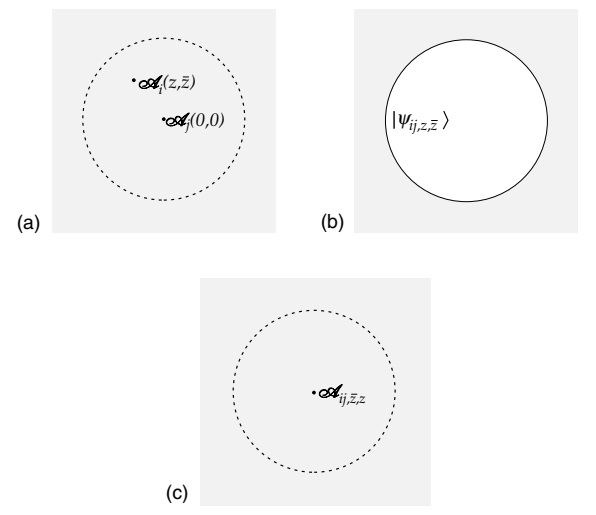
\includegraphics[width=0.8\textwidth,natwidth=370,natheight=300]{Fig2.7.jpg}
\caption{(a) 有两个定域算符的世界面. (b) 对圆盘内的场积分给出边界态$\lvert\psi_{i j, z, \bar{z}}\rangle$. (c) 在有相应定域算符的圆盘内裁切. 展到有确定权的算符上给出 OPE.}\label{Fig2.7}
	\end{center}
\end{figure}
考察乘积
\begin{equation}
\mathscr{A}_{i}(z, \bar{z}) \mathscr{A}_{j}(0,0) \:, \label{2.9.1}
\end{equation}
其中$|z|<1$. 我么可以将路径积分分成对单位圆内部的场$\phi_{\mathrm{i}}$积分, 对单位圆上的场$\phi_{\mathrm{b}}$的积分,对单位圆外部场$\phi_{\mathrm{e}}$的积分. 正如上节末尾所讨论的, 对$\phi_{\mathrm{i}}$的积分给出$\phi_{\mathrm{b}}$的某个泛函, 记其为$\Psi_{i j, z, \bar{z}}[\phi_{\mathrm{b}}]$. 通过态--算符对应, 这等价于将圆盘与合适的算符$\mathscr{A}$ 粘在一起. 为了将其变成以$L_{0}, \tilde{L}_{0}$本征态完备集做展开的标准形式
\begin{equation}
\mathscr{A}_{i j, z, \bar{z}}=\sum_{k} z^{h_{k}-h_{i}-h_{j}}\bar{z}^{\tilde{h}_{k}-\tilde{h}_{i}-\tilde{h}_{j} }c^{k}{}_{i j} \mathscr{A}_{k} \:, \label{2.9.2}
\end{equation}
其中$z$相关性与$\bar{z}$相关性像(\ref{2.4.20})中那样由共形权重决定. OPE 的收敛性正是量子力学中一个完备集的收敛性. 只要在$\lvert z^{\prime}\rvert \leq \lvert z\rvert $中没有其他算符, 这个构造就是可能的. 使得我们可以剪出半径$|z|+\epsilon$ 的圆.

对于三个算符
\begin{equation}
\mathscr{A}_{i}(0,0) \mathscr{A}_{j}(1,1) \mathscr{A}_{k}(z, \bar{z}) \:, \label{2.9.3}
\end{equation}
$z\to 0$ OPE的收敛区域$|z|<1$与$z\to 1$ OPE的收敛区域$|1-z|<1$重叠. 那么三重积中$\mathscr{A}_l$ 的系数可以写成包含$c^{l}{}_{i k} 
c^{m}{}_{l j}$ 的求和或包含$c^{l}{}_{j k} c^{m}{}_{li}$ 的求和. 结合性要求这些和相等. 图解表示见图\ref{Fig2.8}.
\begin{figure}[h]
	\begin{center}
		%	\includegraphics[width=0.8\textwidth,bb=0 0 490 192]{Fig2.3ClosedStringCoordinates.jpg}\\
		%1px=0.75pt
		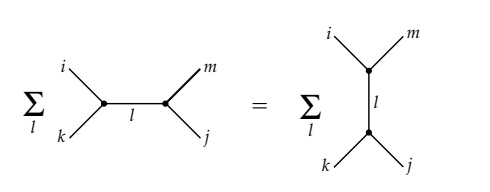
\includegraphics[width=0.8\textwidth,natwidth=300,natheight=110]{Fig2.8.jpg}
		\caption{OPE结合性的图形表示}\label{Fig2.8}
	\end{center}
\end{figure}

\subsection*{Virasoro 代数和最高权重态}

现在对 Virasoro 生成元应用图\ref{Fig2.6}的讨论:
\begin{align}
L_{m}\lvert \mathscr{A}\rangle & \cong \oint \frac{\dif z}{2 \pi \mi}\: z^{m+1} T(z) \mathscr{A}(0,0)  \nonumber \\
& \cong L_{m} \cdot \mathscr{A}(0,0) \:. \label{2.9.4}
\end{align}
这里我们进入了新的记法与概念. 给定态-算符同构, 作用在 Hilbert 空间上的每一算符有一个作用在定域算符空间上的像. 换句话说, 构成了围绕算符的相应围道并利用 OPE 计算出相应的定域算符. 与将态映射到态的$L_m$对应的是是将定域算符映射到定域算符的$L_m\cdot$. 一般而言, 在不同位置$z_i$处会有定域算符, 而每一个位置将有一个 Virasoro 代数的不同版本. 这些不同版本是以算符位置为中心的 Laurent 展开获得的. 在某些几何中也会存在生成元的一个标准基. 例如对于圆柱则以 $z=0$ 为中心的展开. “$\cdot$”充当一个提醒: 我们所讨论的是围绕特定算符的 Laurent 展开系数. 

在这个记法下, $T\mathscr{A}$ OPE 是
\begin{equation}\label{2.9.5}
T(z) \mathscr{A}(0,0)=\sum_{m=-\infty}^{\infty} z^{-m-2} L_{m} \cdot \mathscr{A}(0,0) \:. 
\end{equation}
为了关联到早期记号(\ref{2.4.11})上, 对于$n \geq 0$, $\mathscr{A}^{(n)}=L_{n-1} \cdot \mathscr{A}$, $\mathscr{A}$的共形变换是
\begin{equation}
\delta \mathscr{A}(z, \bar{z})=-\epsilon \sum_{n=0}^{\infty} \frac{1}{n !}\Bigl[\partial^{n} v(z) L_{n-1}+\left(\partial^{n} v(z)\right)^{*} \tilde{L}_{n-1}\Bigr] \cdot \mathscr{A}(z, \bar{z}) \:. \label{2.9.6}
\end{equation}
利用$T\mathscr{A}$ OPE 的一般形式(\ref{2.4.14}), 我们有非常有用的结果
\begin{subequations}\label{2.9.7}
\begin{align}
L_{-1} \cdot \mathscr{A}&=\partial \mathscr{A}, \quad \tilde{L}_{-1} \cdot \mathscr{A}=\bar{\partial} \mathscr{A} \:, \label{2.9.7a} \\
L_{0} \cdot \mathscr{A}&=h \mathscr{A}, \quad \tilde{L}_{0} \cdot \mathscr{A}=\tilde{h} \mathscr{A} \:.\label{2.9.7b}
\end{align}
\end{subequations}
OPE (\ref{2.9.5})暗示了与权重 $(h, \tilde{h})$的基本场$\mathcal{O}$ 对应的态满足
\begin{subequations} \label{2.9.8}
\begin{align}
L_{0}|\mathcal{O}\rangle&=h|\mathcal{O}\rangle \:, \quad \tilde{L}_{0}|\mathcal{O}\rangle=\tilde{h}|\mathcal{O}\rangle \:, \label{2.9.8a} \\
L_{m}|\mathcal{O}\rangle&=\tilde{L}_{m}|\mathcal{O}\rangle=0\:, \quad m>0 \:. \label{2.9.8b}
\end{align}
\end{subequations}
这样的态被称为最高权重态: 通过在任意态上重复作用下降算符, 我们最终会得到被进一步的下降算符湮灭的态, 称为最高权重态. 

一个有趣的特殊情况是单位算符, 算符乘积$T1$是非奇异的, 所以在任意 CFT 中得到
\begin{equation}
L_{m}|1\rangle=\tilde{L}_{m}|1\rangle=0, \quad m \geq-1 \:. \label{2.9.9}
\end{equation}
正如2.4节所标记的, 算符$L_{0}$ 和 $L_{\pm 1}$构成闭代数, $\tilde{L}_{0}$ 和 $\tilde{L}_{\pm 1}$也如此. 整个代数是
\begin{equation}
SL(2,\mathds{R})\times SL(2,\mathds{R})= S L(2, \mathds{C}) \:. \label{2.9.10}
\end{equation}
因此$|1\rangle$也称为 $SL(2, \mathds{C})$-不变态. 它是唯一一个这样的态, 这是因为(\ref{2.9.7})暗示了任何与 $SL(2, \mathds{C})$-不变态对应的算符$\mathscr{A}$都独立于位置, 所以必须是$c$-数, 正如(\ref{2.4.24})之后所解释的. 

\subsection*{幺正 CFT}

最高权重态在弦论以及 Virasoro 代数的表示论中扮演了重要的角色. 现在我们要导出几个在幺正 CFT 中普遍成立的重要结果. 幺正 CFT 有正定内积, 这使得
\begin{equation}
L_{m}^{\dagger}=L_{-m} \: , \quad \tilde{L}_{m}^{\dagger}=\tilde{L}_{-m} \:. \label{2.9.11}
\end{equation}
回忆: 内积经由$\langle\alpha \vert A \beta\rangle=\langle A^{\dagger} \alpha \vert \beta\rangle$ 定义了伴随(adjoint). 
例如$X^\mu$ CFT 对于\emph{类空}的$\mu$是幺正的. 如果我们取基态的内积为
\begin{equation}
\langle 0 ; k \vert 0 ; k^{\prime} \rangle=2 \pi \delta(k-k^{\prime})  \label{2.9.12}
\end{equation} 
并定义
\begin{equation}
\alpha_{m}^{\dagger}=\alpha_{-m} \:, \quad \tilde{\alpha}_{m}^{\dagger}=\tilde{\alpha}_{-m} \:. \label{2.9.13}
\end{equation}
这隐含定义了所有更高态的内积. 这个 CFT 对于$X^\mu=0$不是幺正的, 这是因为那里的对易关系存在一个负号. 

幺正CFT中的第一个约束是任何态都必须有$h, \tilde{h} \geq 0$. 如果这对于最高权重态成立, 那么对所有态成立. 对于最高权重态, Virasoro 代数给出
\begin{equation}\label{2.9.14}
2 h_{\mathcal{O}}\langle\mathcal{O} \vert \mathcal{O}\rangle=2\langle\mathcal{O}\vert L_{0}\vert \mathcal{O}\rangle=\langle\mathcal{O}|[L_{1}, L_{-1}]|\mathcal{O}\rangle=\| L_{-1}|\mathcal{O}\rangle \|^{2} \geq 0 \:,
\end{equation}
所以$h_{\mathcal{O}} \geq 0 $. 如果 $h_{\mathcal{O}}=\tilde{h}_{\mathcal{O}}=0$, 那么
\begin{equation}
L_{-1} \cdot \mathcal{O}=\tilde{L}_{-1} \cdot \mathcal{O}=0 \:, \label{2.9.15}
\end{equation}
因而 $\mathcal{O}$是独立于位置的. 正如之前所标注的, $\mathcal{O}$必须是$c$数, 即在幺正 CFT 中单位算符是唯一$(0,0)$算符. 惊奇的是, $X^\mu$是唯一的例外: 相对应的态$x^{\mu}|0 ; 0\rangle$ 由于 $X^\mu$的无限范围是不归一的, 并且方程(\ref{2.9.14}) 不再成立. 
对于与紧致维对应的 CFT, 一般定理最有用, 这类例外不可能发生.

以同样的方式, 在幺正 CFT 中, 当且仅当$\tilde{h}=0$, 算符才是全纯的, 当且仅当$h=0$, 算符才是反全纯的; 这是一个重要结果, 我们重复如下:
\begin{equation}
\partial \mathscr{A}=0 \Leftrightarrow h=0 \:, \quad \bar{\partial} \mathscr{A}=0 \Leftrightarrow \tilde{h}=0 \:. \label{2.9.16}
\end{equation}
最后, 利用前面的讨论以及对易子$\left[L_{n}, L_{-n}\right]$可以证明在幺正CFT中$c, \tilde{c} \geq 0$. 实际上, $c=0$的唯一幺正CFT是平庸的: $L_n=0$. 

\subsection*{零点能}
态-算符映射给出了另一种不同正规编序常数的简单推导. 在任何 CFT 中, 我们知道$L_{0}|1\rangle=0$, 而这决定了$L_0$ 的又一归一化.
在$X$ CFT中, $|1\rangle=0$是基态, 所以$a^X=0$. 在$bc$理论中, $|1\rangle=0$是激发态$b_{-1}\lvert \downarrow\rangle$, 所以为了与早期$\lambda=2$的结果(\ref{2.7.1}) 一致,  $\lvert \downarrow\rangle$的权重是$-1$.

这也提供了中心荷的物理解释. 在幺正 CFT 中, 基态是$L_{0}=\tilde{L}_{0}=0$的$|1\rangle$. 
径向生成元与时间平移生成元之间的共形变换(\ref{2.6.10})暗示了, 对于基态
\begin{equation}
E=-\frac{c+\tilde{c}}{24} \:. \label{2.9.17}
\end{equation}
这是 Casimir 能量, 源于系统的有限尺度, 且依赖于中心荷. 基于量纲分析, 这个能量反比于系统的尺寸$\ell$, 在这里是$2\pi$, 所以一般结果是
\begin{equation}
E=-\frac{\pi(c+\tilde{c})}{12 \ell} \:. \label{2.9.18}
\end{equation}
我们现在有三种计算正规序列常数的方式:
\begin{enumerate}
	\item 像(\ref{2.7.8})中那样, 从 Virasoro 代数出发;
	\item 像(\ref{2.7.11})中那样, 将正规编序的两种形式关联起来;
	\item 从前面的态-算符映射出发.
\end{enumerate}
然而把零点能加起来的方法是直观的, 所以我们给出另一种描述:
\begin{enumerate}
	\item 对于每个玻色模, 零点能为$\frac{1}{2} \omega$;对于每个费米模, 零点能为$-\frac{1}{2} \omega$. 将能量加起来.
	\item 遇见形如$\sum_{n=1}^{\infty}(n-\theta)$的发散和,  $\theta$源于非平庸的周期条件, 定义其为
	\begin{equation}
	\sum_{n=1}^{\infty}(n-\theta)=\frac{1}{24}-\frac{1}{8}(2 \theta-1)^{2} \:. \label{2.9.19}
	\end{equation}
	这一值可以像\eqref{1.3.32}中那样, 通过正规化并抛弃掉平方发散部分获得.
	\item 前面给出了$w$参考系下生成元$T_0$的正规编序常数, $T_0$由(\ref{2.6.8})给出. 对于$L_0$我们必须加上非张量修正$\frac{1}{24} c$.
\end{enumerate}
对于自由玻色场, 模是整数值, 所以在第2步之后, 对于$\theta=0$, 我们得到了求和的一半, 其是$-\frac{1}{24} $. 这恰好被第3步的修正抵消, 给出$a^X=0$. 对于鬼场, 我们类似地得到$\frac{2}{24}-\frac{26}{24}=-1$.
